
%% This style is provided exclusively for the ICSE 2012 main conference,
%% ICSE 2012 co-located events, and ICSE 2012 workshops.

%% bare_conf_ICSE12.tex
%% V1.4
%% 2012-01-21
%%

%% This is a skeleton file demonstrating the use of IEEEtran.cls
%% (requires IEEEtran.cls version 1.7 or later) with an IEEE conference paper.
%%
%% Support sites:
%% http://www.michaelshell.org/tex/ieeetran/
%% http://www.ctan.org/tex-archive/macros/latex/contrib/IEEEtran/
%% and
%% http://www.ieee.org/

%%*************************************************************************
%% Legal Notice: 
%% This code is offered as-is without any warranty either expressed or
%% implied; without even the implied warranty of MERCHANTABILITY or
%% FITNESS FOR A PARTICULAR PURPOSE! 
%% User assumes all risk.
%% In no event shall IEEE or any contributor to this code be liable for
%% any damages or losses, including, but not limited to, incidental,
%% consequential, or any other damages, resulting from the use or misuse
%% of any information contained here. 
%%
%% All comments are the opinions of their respective authors and are not
%% necessarily endorsed by the IEEE.
%%
%% This work is distributed under the LaTeX Project Public License (LPPL)
%% ( http://www.latex-project.org/ ) version 1.3, and may be freely used,
%% distributed and modified. A copy of the LPPL, version 1.3, is included
%% in the base LaTeX documentation of all distributions of LaTeX released
%% 2003/12/01 or later.
%% Retain all contribution notices and credits.
%% ** Modified files should be clearly indicated as such, including  **
%% ** renaming them and changing author support contact information. **
%%
%% File list of work: IEEEtran.cls, IEEEtran_HOWTO.pdf, bare_adv.tex,
%%                    bare_conf.tex, bare_jrnl.tex, bare_jrnl_compsoc.tex
%%*************************************************************************

% *** Authors should verify (and, if needed, correct) their LaTeX system  ***
% *** with the testflow diagnostic prior to trusting their LaTeX platform ***
% *** with production work. IEEE's font choices can trigger bugs that do  ***
% *** not appear when using other class files.                            ***
% The testflow support page is at:
% http://www.michaelshell.org/tex/testflow/



% Note that the a4paper option is mainly intended so that authors in
% countries using A4 can easily print to A4 and see how their papers will
% look in print - the typesetting of the document will not typically be
% affected with changes in paper size (but the bottom and side margins will).
% Use the testflow package mentioned above to verify correct handling of
% both paper sizes by the user's LaTeX system.
%
% Also note that the "draftcls" or "draftclsnofoot", not "draft", option
% should be used if it is desired that the figures are to be displayed in
% draft mode.
%
%\documentclass[10pt, conference, compsocconf]{IEEEtran}
\documentclass[conference]{IEEEtran}

% Add the compsocconf option for Computer Society conferences.
%
% If IEEEtran.cls has not been installed into the LaTeX system files,
% manually specify the path to it like:
% \documentclass[conference]{../sty/IEEEtran}


\usepackage{balance}
\usepackage{float}

% Some very useful LaTeX packages include:
% (uncomment the ones you want to load)


% *** MISC UTILITY PACKAGES ***
%
%\usepackage{ifpdf}
% Heiko Oberdiek's ifpdf.sty is very useful if you need conditional
% compilation based on whether the output is pdf or dvi.
% usage:
% \ifpdf
%   % pdf code
% \else
%   % dvi code
% \fi
% The latest version of ifpdf.sty can be obtained from:
% http://www.ctan.org/tex-archive/macros/latex/contrib/oberdiek/
% Also, note that IEEEtran.cls V1.7 and later provides a builtin
% \ifCLASSINFOpdf conditional that works the same way.
% When switching from latex to pdflatex and vice-versa, the compiler may
% have to be run twice to clear warning/error messages.






% *** CITATION PACKAGES ***
%
%\usepackage{cite}
% cite.sty was written by Donald Arseneau
% V1.6 and later of IEEEtran pre-defines the format of the cite.sty package
% \cite{} output to follow that of IEEE. Loading the cite package will
% result in citation numbers being automatically sorted and properly
% "compressed/ranged". e.g., [1], [9], [2], [7], [5], [6] without using
% cite.sty will become [1], [2], [5]--[7], [9] using cite.sty. cite.sty's
% \cite will automatically add leading space, if needed. Use cite.sty's
% noadjust option (cite.sty V3.8 and later) if you want to turn this off.
% cite.sty is already installed on most LaTeX systems. Be sure and use
% version 4.0 (2003-05-27) and later if using hyperref.sty. cite.sty does
% not currently provide for hyperlinked citations.
% The latest version can be obtained at:
% http://www.ctan.org/tex-archive/macros/latex/contrib/cite/
% The documentation is contained in the cite.sty file itself.






% *** GRAPHICS RELATED PACKAGES ***
%
\ifCLASSINFOpdf
  \usepackage[pdftex]{graphicx}
  % declare the path(s) where your graphic files are
  \graphicspath{{../pdf/}{../jpeg/}}
  % and their extensions so you won't have to specify these with
  % every instance of \includegraphics
  \DeclareGraphicsExtensions{.pdf,.jpeg,.png}
\else
  % or other class option (dvipsone, dvipdf, if not using dvips). graphicx
  % will default to the driver specified in the system graphics.cfg if no
  % driver is specified.
  \usepackage[dvips]{graphicx}
  % declare the path(s) where your graphic files are
  \graphicspath{{../eps/}}
  % and their extensions so you won't have to specify these with
  % every instance of \includegraphics
  \DeclareGraphicsExtensions{.eps}
\fi
% graphicx was written by David Carlisle and Sebastian Rahtz. It is
% required if you want graphics, photos, etc. graphicx.sty is already
% installed on most LaTeX systems. The latest version and documentation can
% be obtained at: 
% http://www.ctan.org/tex-archive/macros/latex/required/graphics/
% Another good source of documentation is "Using Imported Graphics in
% LaTeX2e" by Keith Reckdahl which can be found as epslatex.ps or
% epslatex.pdf at: http://www.ctan.org/tex-archive/info/
%
% latex, and pdflatex in dvi mode, support graphics in encapsulated
% postscript (.eps) format. pdflatex in pdf mode supports graphics
% in .pdf, .jpeg, .png and .mps (metapost) formats. Users should ensure
% that all non-photo figures use a vector format (.eps, .pdf, .mps) and
% not a bitmapped formats (.jpeg, .png). IEEE frowns on bitmapped formats
% which can result in "jaggedy"/blurry rendering of lines and letters as
% well as large increases in file sizes.
%
% You can find documentation about the pdfTeX application at:
% http://www.tug.org/applications/pdftex





% *** MATH PACKAGES ***
%
%\usepackage[cmex10]{amsmath}
% A popular package from the American Mathematical Society that provides
% many useful and powerful commands for dealing with mathematics. If using
% it, be sure to load this package with the cmex10 option to ensure that
% only type 1 fonts will utilized at all point sizes. Without this option,
% it is possible that some math symbols, particularly those within
% footnotes, will be rendered in bitmap form which will result in a
% document that can not be IEEE Xplore compliant!
%
% Also, note that the amsmath package sets \interdisplaylinepenalty to 10000
% thus preventing page breaks from occurring within multiline equations. Use:
%\interdisplaylinepenalty=2500
% after loading amsmath to restore such page breaks as IEEEtran.cls normally
% does. amsmath.sty is already installed on most LaTeX systems. The latest
% version and documentation can be obtained at:
% http://www.ctan.org/tex-archive/macros/latex/required/amslatex/math/





% *** SPECIALIZED LIST PACKAGES ***
%
%\usepackage{algorithmic}
% algorithmic.sty was written by Peter Williams and Rogerio Brito.
% This package provides an algorithmic environment fo describing algorithms.
% You can use the algorithmic environment in-text or within a figure
% environment to provide for a floating algorithm. Do NOT use the algorithm
% floating environment provided by algorithm.sty (by the same authors) or
% algorithm2e.sty (by Christophe Fiorio) as IEEE does not use dedicated
% algorithm float types and packages that provide these will not provide
% correct IEEE style captions. The latest version and documentation of
% algorithmic.sty can be obtained at:
% http://www.ctan.org/tex-archive/macros/latex/contrib/algorithms/
% There is also a support site at:
% http://algorithms.berlios.de/index.html
% Also of interest may be the (relatively newer and more customizable)
% algorithmicx.sty package by Szasz Janos:
% http://www.ctan.org/tex-archive/macros/latex/contrib/algorithmicx/




% *** ALIGNMENT PACKAGES ***
%
%\usepackage{array}
% Frank Mittelbach's and David Carlisle's array.sty patches and improves
% the standard LaTeX2e array and tabular environments to provide better
% appearance and additional user controls. As the default LaTeX2e table
% generation code is lacking to the point of almost being broken with
% respect to the quality of the end results, all users are strongly
% advised to use an enhanced (at the very least that provided by array.sty)
% set of table tools. array.sty is already installed on most systems. The
% latest version and documentation can be obtained at:
% http://www.ctan.org/tex-archive/macros/latex/required/tools/


%\usepackage{mdwmath}
%\usepackage{mdwtab}
% Also highly recommended is Mark Wooding's extremely powerful MDW tools,
% especially mdwmath.sty and mdwtab.sty which are used to format equations
% and tables, respectively. The MDWtools set is already installed on most
% LaTeX systems. The lastest version and documentation is available at:
% http://www.ctan.org/tex-archive/macros/latex/contrib/mdwtools/


% IEEEtran contains the IEEEeqnarray family of commands that can be used to
% generate multiline equations as well as matrices, tables, etc., of high
% quality.


%\usepackage{eqparbox}
% Also of notable interest is Scott Pakin's eqparbox package for creating
% (automatically sized) equal width boxes - aka "natural width parboxes".
% Available at:
% http://www.ctan.org/tex-archive/macros/latex/contrib/eqparbox/





% *** SUBFIGURE PACKAGES ***
%\usepackage[tight,footnotesize]{subfigure}
% subfigure.sty was written by Steven Douglas Cochran. This package makes it
% easy to put subfigures in your figures. e.g., "Figure 1a and 1b". For IEEE
% work, it is a good idea to load it with the tight package option to reduce
% the amount of white space around the subfigures. subfigure.sty is already
% installed on most LaTeX systems. The latest version and documentation can
% be obtained at:
% http://www.ctan.org/tex-archive/obsolete/macros/latex/contrib/subfigure/
% subfigure.sty has been superceeded by subfig.sty.



%\usepackage[caption=false]{caption}
%\usepackage[font=footnotesize]{subfig}
% subfig.sty, also written by Steven Douglas Cochran, is the modern
% replacement for subfigure.sty. However, subfig.sty requires and
% automatically loads Axel Sommerfeldt's caption.sty which will override
% IEEEtran.cls handling of captions and this will result in nonIEEE style
% figure/table captions. To prevent this problem, be sure and preload
% caption.sty with its "caption=false" package option. This is will preserve
% IEEEtran.cls handing of captions. Version 1.3 (2005/06/28) and later 
% (recommended due to many improvements over 1.2) of subfig.sty supports
% the caption=false option directly:
%\usepackage[caption=false,font=footnotesize]{subfig}
%
% The latest version and documentation can be obtained at:
% http://www.ctan.org/tex-archive/macros/latex/contrib/subfig/
% The latest version and documentation of caption.sty can be obtained at:
% http://www.ctan.org/tex-archive/macros/latex/contrib/caption/




% *** FLOAT PACKAGES ***
%
%\usepackage{fixltx2e}
% fixltx2e, the successor to the earlier fix2col.sty, was written by
% Frank Mittelbach and David Carlisle. This package corrects a few problems
% in the LaTeX2e kernel, the most notable of which is that in current
% LaTeX2e releases, the ordering of single and double column floats is not
% guaranteed to be preserved. Thus, an unpatched LaTeX2e can allow a
% single column figure to be placed prior to an earlier double column
% figure. The latest version and documentation can be found at:
% http://www.ctan.org/tex-archive/macros/latex/base/



%\usepackage{stfloats}
% stfloats.sty was written by Sigitas Tolusis. This package gives LaTeX2e
% the ability to do double column floats at the bottom of the page as well
% as the top. (e.g., "\begin{figure*}[!b]" is not normally possible in
% LaTeX2e). It also provides a command:
%\fnbelowfloat
% to enable the placement of footnotes below bottom floats (the standard
% LaTeX2e kernel puts them above bottom floats). This is an invasive package
% which rewrites many portions of the LaTeX2e float routines. It may not work
% with other packages that modify the LaTeX2e float routines. The latest
% version and documentation can be obtained at:
% http://www.ctan.org/tex-archive/macros/latex/contrib/sttools/
% Documentation is contained in the stfloats.sty comments as well as in the
% presfull.pdf file. Do not use the stfloats baselinefloat ability as IEEE
% does not allow \baselineskip to stretch. Authors submitting work to the
% IEEE should note that IEEE rarely uses double column equations and
% that authors should try to avoid such use. Do not be tempted to use the
% cuted.sty or midfloat.sty packages (also by Sigitas Tolusis) as IEEE does
% not format its papers in such ways.





% *** PDF, URL AND HYPERLINK PACKAGES ***
%
%\usepackage{url}
% url.sty was written by Donald Arseneau. It provides better support for
% handling and breaking URLs. url.sty is already installed on most LaTeX
% systems. The latest version can be obtained at:
% http://www.ctan.org/tex-archive/macros/latex/contrib/misc/
% Read the url.sty source comments for usage information. Basically,
% \url{my_url_here}.





% *** Do not adjust lengths that control margins, column widths, etc. ***
% *** Do not use packages that alter fonts (such as pslatex).         ***
% There should be no need to do such things with IEEEtran.cls V1.6 and later.
% (Unless specifically asked to do so by the journal or conference you plan
% to submit to, of course. )


% correct bad hyphenation here
\hyphenation{op-tical net-works semi-conduc-tor}


\begin{document}
%
% paper title
% can use linebreaks \\ within to get better formatting as desired
\title{Mining the Temporal Evolution of the Android Bug Reporting
  Community \\ via Sliding Windows}


% author names and affiliations
% use a multiple column layout for up to two different
% affiliations

\author{\IEEEauthorblockN{\quad \quad \quad \quad \quad Feng Jiang, Jiemin Wang, Abram Hindle, Mario A. Nascimento}
\IEEEauthorblockA{\quad \quad \quad \quad \quad Department of Computing Science\\
\quad \quad \quad \quad \quad University of Alberta\\
\quad \quad \quad \quad \quad Edmonton, Alberta, Canada\\
\quad \quad \quad \quad \quad \{fjiang2, jiemin2, abram.hindle, mario.nascimento\}@ualberta.ca}
\and

}

% conference papers do not typically use \thanks and this command
% is locked out in conference mode. If really needed, such as for
% the acknowledgment of grants, issue a \IEEEoverridecommandlockouts
% after \documentclass

% for over three affiliations, or if they all won't fit within the width
% of the page, use this alternative format:
% 
%\author{\IEEEauthorblockN{Michael Shell\IEEEauthorrefmark{1},
%Homer Simpson\IEEEauthorrefmark{2},
%James Kirk\IEEEauthorrefmark{3}, 
%Montgomery Scott\IEEEauthorrefmark{3} and
%Eldon Tyrell\IEEEauthorrefmark{4}}
%\IEEEauthorblockA{\IEEEauthorrefmark{1}School of Electrical and Computer Engineering\\
%Georgia Institute of Technology,
%Atlanta, Georgia 30332--0250\\ Email: see http://www.michaelshell.org/contact.html}
%\IEEEauthorblockA{\IEEEauthorrefmark{2}Twentieth Century Fox, Springfield, USA\\
%Email: homer@thesimpsons.com}
%\IEEEauthorblockA{\IEEEauthorrefmark{3}Starfleet Academy, San Francisco, California 96678-2391\\
%Telephone: (800) 555--1212, Fax: (888) 555--1212}
%\IEEEauthorblockA{\IEEEauthorrefmark{4}Tyrell Inc., 123 Replicant Street, Los Angeles, California 90210--4321}}




% use for special paper notices
%\IEEEspecialpapernotice{(Invited Paper)}




% make the title area
\maketitle


\begin{abstract}
% need to be expanded !!!

The open source development community consists of both paid and volunteer
developers as well as new and experienced users.
Previous work has applied social network analysis (SNA) to open source
communities and has demonstrated value in expertise discovery and
triaging. 
One problem of applying SNA directly to the data of the whole time period is that the impact of local activities will probably be drowned out. In this paper we provide a method for aggregating, analyzing, and visualizing local (small time periods) interactions of bug reporting participants by
using the SNA to measure the betweeness centrality of these participants.
In particular we mined the Android bug repository by producing 
social networks from the 30-day windows of bug reports, each sliding
over by day.
In this paper we define three patterns of participant
behaviour based on their local centrality. We propose a method of analyzing centrality of bug
report participants both locally and globally, with which we conduct a thorough case study of the bug reporters' activity within the Android
bug repository.
Further, we validate the conclusions of our method by mining the Android version control system.


\end{abstract}

\begin{IEEEkeywords}
mining software repository; social network analysis; sliding windows

\end{IEEEkeywords}


% For peer review papers, you can put extra information on the cover
% page as needed:
% \ifCLASSOPTIONpeerreview
% \begin{center} \bfseries EDICS Category: 3-BBND \end{center}
% \fi
%
% For peerreview papers, this IEEEtran command inserts a page break and
% creates the second title. It will be ignored for other modes.
\IEEEpeerreviewmaketitle



\section{Introduction}
% two columns !!!

\label{introduction}
% no \IEEEPARstart

%XXX cite
% Introduce SNA
% Introduce bug repository
% Social network analysis (SNA) is a powerful tool that helps
% practioners and researchers study the complicated interactions of
% participants within communities, SNA analysis is well accepted within
% the software maintenance and mining software repositories communities.
% SNA allows us to study the structure of the interactions between software developers and users
% within a software project's community using graph metrics on the graph
% of discussions that occur in the bug repository.
% Since the interaction in the communities records the activities of
% each participant and the communication among them


%SNA
\emph{Social network analysis} (SNA) is a powerful tool that helps
practitioners and researchers study the complicated interactions of
participants within communities, SNA is well accepted in the area of software maintenance and mining software repositories
communities~\cite{CAMB:wass,MSR:christ,ICSEsocio:meneely}.  
%
The bug repository records interactions among software developers and users in a software
project's community. With SNA, we are able to study the structure of the interactions by analysing the graph constructed for the bug repository.
%
The conclusions can be used in expertise elicitation and
triaging to indicate which  participants have expertise relevant
to an issue~\cite{ICSEsocio:meneely}. 


Open-source communities are amenable to social network analysis as
they are
open to user interaction and participation. 
At the same time there is a lack of imposed organizational
structures view within corporate organizations~\cite{ACM:chris}.
Because open source projects often lack strict centralized control and
requirements~\cite{AMCIS:Freeh}, developers often choose their
tasks instead of being assigned one~\cite{ACM:ashish}. 
This fact suggests that local structure of interactions among users and developers
who have an interest in one part of the project tend to self
organize, which resulting in interesting collaboration structures (networks).


%Bug repos
Bug repositories are also amenable to social network analysis as bug
repositories host and record discussions regarding issues or bugs relevant to
the development and the use of a software development
project~\cite{ACM:ashish,OSD:yasu}. 
Bug repositories are also very popular among open-source projects.
Collaboration among developers has been studied in various aspects about how the communication introduces or avoids bugs, and further influences the software quality, \cite{CSMR:bernardi}, \cite{ACM:abreu}, \cite{ACM:pinzger}, \cite{IEEE:bettenburg}. 
Besides the collaboration among developers, collaboration between users and developers is evident in bug
reports since the discussions and communications are recorded as reported bugs, and posted comments
on bug reports.


%In this paper, we studied the Android bug community. The Android development contains both the systems or the sdks and the apps; it covers varieties of technique topics, and at the same time, developers are not organized statically as the very standard commercial software. The Android development comprises participants from different vanders, for example, some are from Motorola, some are from HTC, or Samsung, etc, and thus it should be interesting and worthwhile to study the Android community and see how well it could relate to the development facts. 

% Bug participants
In the case of the Android bug repository, provided by the 2012 MSR
Mining Challenge~\cite{DATA:msr}, a reporter would report a bug, which
might attract comments from bug commenters. The commenters discuss the
reasons and possible resolution of the bug.
The bug reporting community members are usually comprised of both bug
reporters and bug commenters who are either Android developers or
Android users.
From the perspective of the bug repository, unlike the version control
system, there is actually no
obvious boundary between a user and a developer.
We refer to these different participants as \emph{bug participants}.

% Setup SNA
In order to apply SNA to the bug repository, we first create the graph based on the interactions. 
We pose that each node of the graph represents
one bug participant and each edge represents the connection between
two participants who have discussed on the same bug. 
We will introduce the network graphs in detail in
Section ~\ref{methodology}.

% SNA Metric
We use betweenness centrality to quantify the importance of a
participant in the community \cite{ICSEsocio:la} 
(betweenness centrality will be better explained in 
 Section ~\ref{methodology}).
The betweenness centrality could reveal two aspects of a participant
in a community network: 1) the quantity of bug reports (which attract
at least one comment) or comments they have made and 2) the importance
of the content of their reports or comments. 
When participants have high betweenness, they might have: 1) reported
quantities of bugs with at least one comment on them, 2) made lots of
comments, 3) reported a very critical bug, 4) or made a very
interesting comment which attracts comments from other participants.


% Previous work which applied SNA to software development has been
% introduced such as mining email archives and mining defect tracking
% systems \cite{MSR:christ} \cite{ACM:ashish} \cite{OSD:yasu}. 
% Similarly, we built our SNA on bug reporting repository, which
% includes both bug reports and comments, and looked into the Android
% bug community based on the participants' activities and discussions.

% But we use windows
However, the previous work~\cite{MSR:christ,ACM:ashish} applied 
SNA on the entire lifetime of a project, such that only a single community network was constructed. 
Some of these collaborations might not be evident if one were to
analyze a large single network.
That is because certain structures will not be observable on the global scale.
In order to peer into these local self organized structures using
social network analysis, we felt it's better to choose a windowed approach, \cite{ICSEsocio:meneely}
\cite{ICSMwindowed:hindle}. 
Windowing allows us to look at network during a slice of time
and then relate our measures (betweenness centrality per author) to
the next window and beyond. 
This sliding window view of centrality allows us to see those
developers and users who are constantly at the forefront of discussion or
those who and ebb and flow between issues and tasks.
Moreover, by sliding windows, each pair of adjacent windows would have
an overlap, which results in smoother trends, and more importantly,
helps to maintain context. 
Other benefits provided by time windowed analysis is that it gives a more accurate and nuanced view of the data as 
locally central participants then will not be 
``drowned out''.




% In this case, the results would only reflect a static view, but ignore
% the trends and changing patterns of the community structures and the
% participants' social characters. 
% Thus, in this paper, we adopt the time windowed method so that we are
% able to analyze the changes along the time line. 
% Other benefits provided by time windowed analysis is that it could
% give a more accurate and nuanced view of the data
% \cite{ICSEsocio:meneely} \cite{ICSMwindowed:hindle}. 

% % And we validate
% We also seek to validate if this windowed methodology actually
% highlights relevant behaviour.
% % Further, as mentioned above, when applying SNA to study the software
% % community, we expect a match between the hypothesis we made from the
% % mining results and the facts in real development process. 
% To help validate if this method highlights existing relevant behaviour 
% we inspected the Android release
% history\footnote[1]{Android release history:
%   http://developer.android.com/sdk/index.html} and the Android changes
% repository.
% % both of which reflect the real development activities.
% % We study the change records authored by bug participants (those who
% % have submissions in the version control system) to get the technique
% % specialties and the type of tasks they were working on. 
% %The participants we selected are those who ever show high betweenness
% %centrality or have characterized activity patterns along the time
% %line. 
% %By inspecting the Android release history, we get the contents of each
% %major or minor releases. 
% More details about the validation would be explained in Section
% \ref{validation}.

<<<<<<< HEAD
=======
We also seek to validate if this windowed methodology actually
highlights relevant behaviour.
To help validate if this method highlights existing relevant behaviour 
we inspected the Android release
history\footnote[1]{Android release history:
  http://developer.android.com/sdk/index.html} and the Android version
control system.
More details about the validation would be explained in Section
\ref{validation}.
 

>>>>>>> 788897dc7945851dec3c2974deb2851042e0fbd1
In summary, we use SNA to study the activities of bug
participants based on the Android bug reports and comments
repository. 
We apply the sliding window method to observe smooth change trends
in the collaboration graph across time.
With these mining results, we seek to analyze bug participants'
interactions, activity trends and patterns. 
We then demonstrate our analysis results via answering the following
research questions about local and global behaviours.


Globally:

\textbf{RQ1.} How does the number of active bug participants change over
  time? Why?

\textbf{RQ2.} How does the betweenness centrality of a participant change over
time? What are the reasons when they have a certain activity pattern?

Locally:

\textbf{RQ3.} Are there special time ranges during which participants are more/less
active or central than normal? Why?

\textbf{RQ4.} What are the possible scenarios for a very sharp change of the
participants' centrality? Why?

Further, we also validate if this windowed methodology actually
highlights relevant behaviour.
To help validate if this method highlights existing relevant behaviour 
we inspected the Android release
history\footnote[1]{Android release history:
  http://developer.android.com/sdk/index.html} and the Android version
control system.
The validation would be discussed in Section
\ref{validation}.
 

% 
The rest of our paper is organized as follows. 
Section \ref{background} introduces basic concepts and techniques we
used in this study. 
The specific steps and the methodology will be discussed in Section
\ref{methodology}. 
Section \ref{results} describes the details of our mining results. 
The analysis of the results and its corresponding validation is
provided in Section \ref{validation}. 
Section \ref{limitation} presents the limitations of our mining
process and Section \ref{conclusion} summarizes the paper and
discusses the future work.

%%%%%%%%%%%%%%4. What are the possible scenarios for the very sharp change in the participants' centrality?

% You must have at least 2 lines in the paragraph with the drop letter
% (should never be an issue)
\begin{figure}[!t]
\centerline{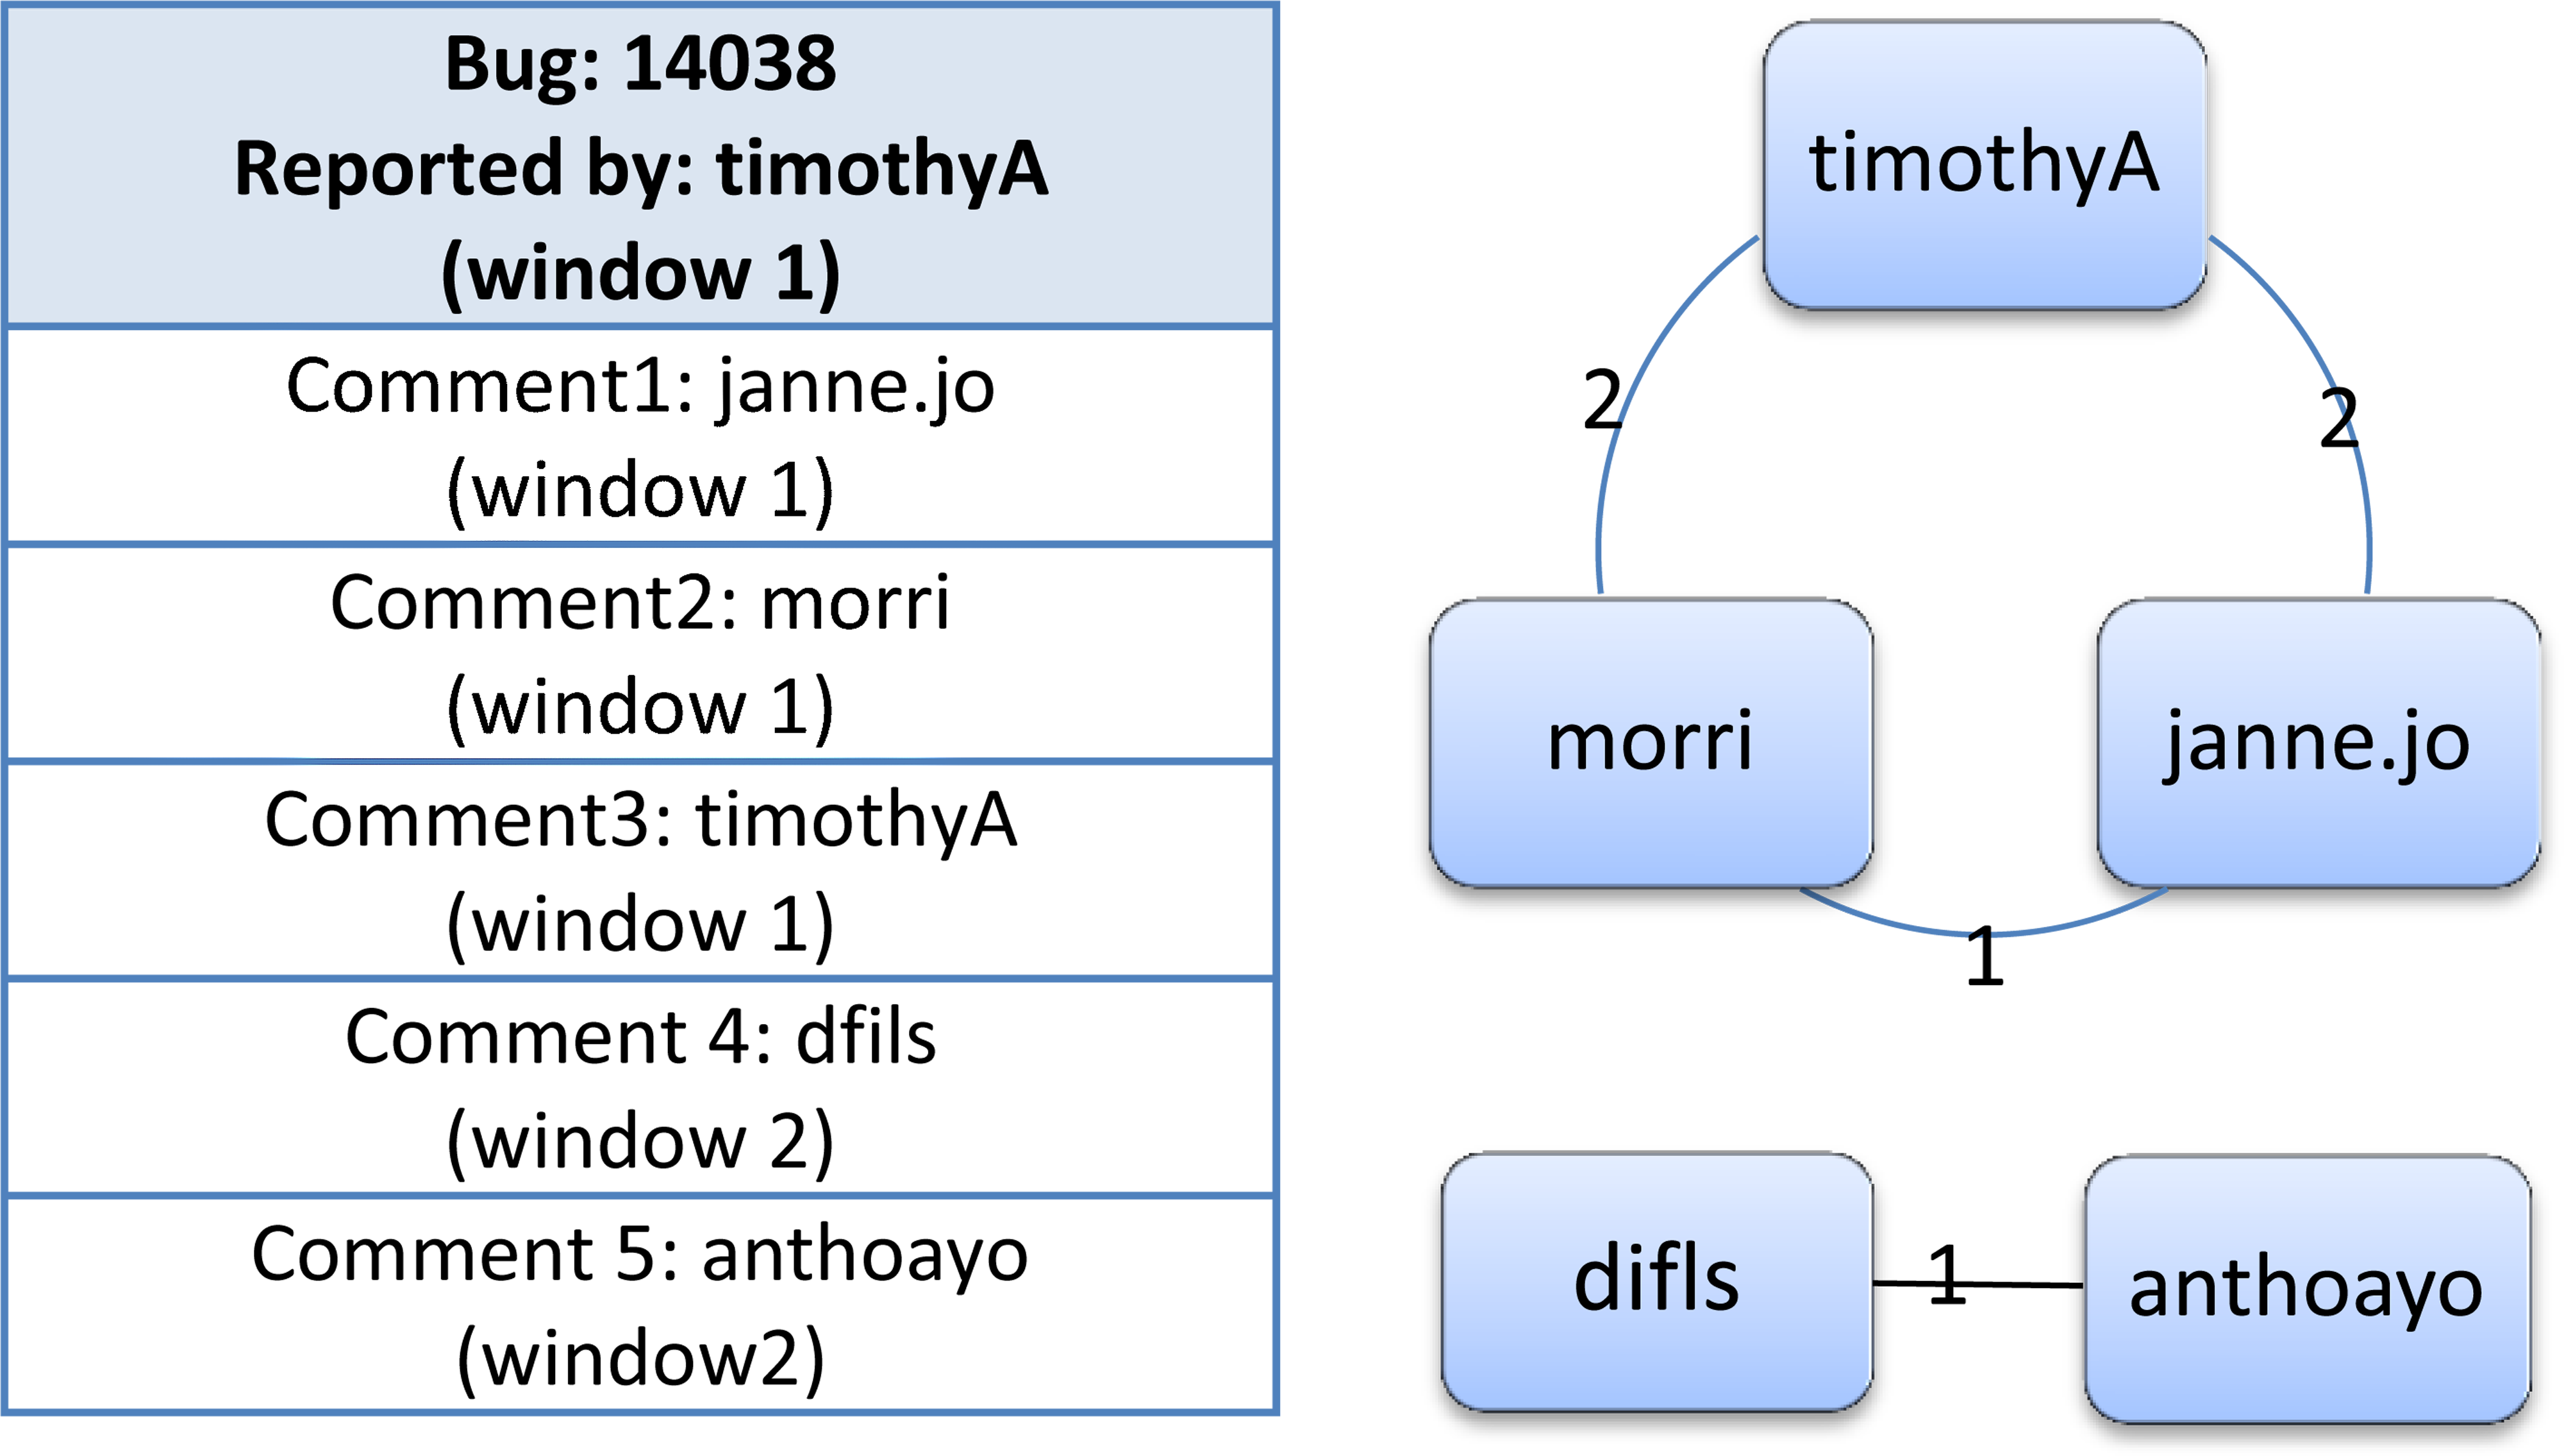
\includegraphics[width=2.6in,height = 3.8cm]{graph.png}
\label{graph}}
\caption{An example: bug 14038 is reported by timothyA, and there are
  five comments on this bug. 
When time window applied, comments are plotted into two windows, and
the bug report of this example forms two networks with the weight
noted on their edges}

\end{figure}

\section{Background}
\label{background}
% talk about window, overlap, cluster 
% need to take up 2 columns
\subsection{Betweenness Centrality}

% XXX Defined by Freeman? Link/Cite!
<<<<<<< HEAD
The betweenness centrality of
=======
The betweenness centrality~\footnote[2]{Centrality:
  http://en.wikipedia.org/wiki/Centrality (March 2012)} of
>>>>>>> 788897dc7945851dec3c2974deb2851042e0fbd1
a vertex is the number of geodesic paths in a graph that includes this
vertex;
the geodesic path is defined as the shortest path which has the
minimum weight between two nodes. 
<<<<<<< HEAD
Defined by Freeman \cite{SOCIO:freeman}, the betweenness can be represented as:
=======
Defined by Freeman, the betweenness can be represented as:
>>>>>>> 788897dc7945851dec3c2974deb2851042e0fbd1

\begin{equation} 
\sum_{i=1}^{j-1}\sum_{j=1}^{n}\frac{g_{ij}(k)}{g_{ij}}, i\neq j \neq k
\end{equation}

<<<<<<< HEAD
where $k$ is a vertex of the graph, $n$ is the total number of
vertices, $i$ and $j$ are vertices other than $k$, $g_{ij}$ is the
number of geodesic paths between vertex $i$ and $j$, and $g_{ij}(k)$
is the number of geodesic paths that include $k$.


It is used as a measurement of a person's importance in a network. 
A person would be regarded as central if he is on the geodesic path
between two other persons. 
As proposed by Freeman, if a person is located
on the geodesic path between two other persons, he becomes one of the key
persons who connects the others. 
That is, the more a person connects to
the other people in a network, the more important or central he is~\cite{BOOK:han}.


In our work, we normalize the betweenness centrality values to eliminate the effect of different sizes of the
networks. The betweenness is normalized as:

\begin{equation}
\label{normalizedb}
Normalized-B = \frac{B}{\frac{(n-1)(n-2)}{2}}
\end{equation} 

where $B$ represents the original betweenness value and n is the number of nodes in the graph being calculated.

Compared with simply counting the total number of comments or total
bug reports of a participant, betweenness acts better to reflect the
interactions among people. For example, when a person reports lots of
bugs but none of them attract any comment, it is very likely that
his bug reports are not interesting or important. In this case, if
we merely counted the number of their reports or comments, we would
possibly increase their importance in the network
artificially. Therefore, we choose to use betweenness centrality to
eliminate this unfair counting~\cite{ICSEsocio:la}.

\subsection{Overlapping Time Windowing}
\label{overlappingtimewindowing}
When SNA is applied in other
papers~\cite{MSR:christ,ICSEsocio:meneely}, it is typically applied to
the entire history or one period of the partial history and all the
bug reports within that period.
Windowed analysis instead repeats social network analysis across 100s
of windows (in our case, as many windows as we have days). These
windows overlap and often the analysis of one window results in the
same analysis as the previous window due to overlap. We slid our
windows by 1 day and for two adjacent windows
$A$ and $B$, $B$ starts on the second day of $A$, and they would have
an overlap of 29 days, that is each window does
some redundant analysis but this leads to smoother transitions in
analysis between windows. Thus 1 comment in a bug report will have an
effect on the graphs of 30 windows. This is similar to Hindle et
al.'s~\cite{ICSMwindowed:hindle} analysis of topics using windows but
they did not use an overlap. We could thus see the changes or get the trend of a participant's activity along the sliding windows.

Moreover, time windowing analysis could give a more accurate and
nuanced view of the data \cite{ICSEsocio:meneely}
\cite{ICSMwindowed:hindle}, as locally central participants would not
be ``drowned out''. For instance, if a
bug participant participates in many bug reports and bug comments during one
month, he would be one of the most central participants with a high
betweenness within this window. However, if he never appeared except for that
month, globally, he would have low betweenness and would not show up
as central, though during a shorter period he has played a vital role. 
As we can see in Figure 2, the left part shows the betweenness values of participants 
over the entire time period; local details are missed and we get nothing about the trend, compared to the left part of the results from overlapping windowing.


Another point is that, comments on the same bug might not be globally
temporally relevant~\cite{Springer:kidane,Procedia:ibaa} thus 
 a global time analysis would not make much sense in this case. This
 could happen if new changes induce new bugs or change the behaviour
 of a reported bug. Also, if there
is a very sharp drop on values of a certain participant, the
overlapping windows would give a more nuanced view of the change and
what was happening.
=======
where $p_k$ is a vertex of the graph, $n$ is the total number of
vertices, $i$ and $j$ are vertices other than $p_k$, $g_{ij}$ is the
number of geodesic paths between vertex $i$ and $j$, and $g_{ij}(p_k)$
is the number of geodesic paths that include $p_k$.


It is used as a measurement of a person's importance in a network. 
A person would be regarded as central if they are on the geodesic path
between two other persons. 
As proposed by Freeman, if a person is located
on the geodesic path between two other persons, they become the key
person who connects the others. 
That is, the more a person connects to
the other people in a network, the more important or central they 
are~\cite{BOOK:han}.


In our work, we normalize the betweenness centrality values with the
number of node pairs to eliminate the effect of different sizes of the
networks.


Compared with simply counting the total number of comments or total
bug reports of a participant, betweenness acts better to reflect the
interactions among people. For example, when a person reports lots of
bugs but none of them attract any comment, it is very likely that
their bug reports are not interesting or important. In this case, if
we merely counted the number of their reports or comments, we would
possibly increase their importance in the network
artificially. Therefore, we choose to use betweenness centrality to
eliminate this unfair counting~\cite{ICSEsocio:la}.


\subsection{Overlapping Time Windowing}

When SNA is applied in other
papers~\cite{MSR:christ,ICSEsocio:meneely} it is typically applied to
the entire history or one period of the partial history and all the
bug reports within that period.
Windowed analysis instead repeats social network analysis across 100s
of windows (in our case, as many windows as we have days). These
windows overlap and often the analysis of one window results in the
same analysis as the previous window due to overlap. We slid our
windows by 1 day, so our overlap is 29 days, that is each window does
some redundant analysis but this leads to smoother transitions in
analysis between windows. Thus 1 comment in a bug report will have an
effect on the graphs of 30 windows. This is similar to Hindle et
al.'s\cite{ICSMwindowed:hindle} analysis of topics using windows but
they did not use an overlap.

Moreover, time windowing analysis could give a more accurate and
nuanced view of the data \cite{ICSEsocio:meneely}
\cite{ICSMwindowed:hindle}, as locally central participants would not
be ``drowned out''. For instance, if a
bug participant participated in many bug reports and bug comments during one
month from January 1st to January 30th, 2010, within this window, they
would be one of the most central participants with a high
betweenness. However, if they never appeared except for that
month, globally, they would have low betweenness and would not show up
as central
central, though during a shorter period they have played a vital role. 


Another point is that, comments on the same bug might not be globally
temporally relevant~\cite{Springer:kidane,Procedia:ibaa} thus 
 a global time analysis would not make much sense in this case. This
 could happen if new changes induce new bugs or change the behaviour
 of a reported bug.

In this paper, we slide the windows by one day and there
is an overlap between two adjacent windows. For two adjacent windows
$A$ and $B$, $B$ starts on the second day of $A$, and they would have
an overlap of 29 days. Normally, windows could be either
overlapped or not. We choose to use the overlapping window because the
overlapping smooths trends and maintains context. If there
is a very sharp drop on values of a certain participant, the
overlapping windows would give a more nuanced view of the change and
what was happening.


\subsection{Clustering}

In order to perceive clusters, that is local groups of interactions,
we clustered the bug participants by their betweenness centrality
distribution along the time line. 
%XXX cite K-Means
%XXX What is K?
K-means is one of the most popular
clustering methods. 
We choose to use K-means with Cosine distance
since from our own experiments, data clustered by K-means with Cosine
distance gives a better view than K-means with Euclidean
distance. 
In this paper Cosine distance calculates the similarity between each pair
author in terms of temporal centrality whereas Euclidean distance
focuses on the magnitude of data, the size and frequency of centrality.
The
Cosine distance between two vectors could be defined as,


\begin{equation}
Cosine\_dist(A,B) = 1-\frac{A\cdot B}{\Arrowvert A \Arrowvert \Arrowvert B \Arrowvert}
\end{equation}

where A and B are two vectors, $\{\cdot\}$ represents the inner dot
operation and $\Arrowvert \cdot \Arrowvert$ indicates the module of
the vector. With clustering, authors with similar temporal centrality would be
grouped together so that bug participants with similar activity
patterns would also be grouped together.  In this study we used
K-means, where $K =
100$, to cluster authors.


\section{Methodology}
\label{methodology}
\subsection{Data}

With the provided Android bug repository and the Android version
control system
from the MSR Challenge~\cite{DATA:msr}, we converted the XML format data to
a database for efficient analysis using Microsoft SQL Server Business
Intelligence. Our analysis focused on the bug records of the previous
two years from January 1st 2010 to December 4th 2011 since participants
during these two years are more active than the other years and the
activities are representative, as showed in Figure 2. The data we used
covers 14,432 out of 20,169 total bug records and 46,806 out of 67,730
total bug comments. Related to these bug and comment records, there
are 30,969 people who have either reported a bug or made comments on a
bug.


The bug and comment records are grouped into 30-day windows sliding by
1 day. 
%The strategy of taking 30 days as a window and sliding by 1 day
%would be discussed in detail in Section \ref{methodology}. 
We extracted 673 daily windows  from the bug reports we selected.

In addition, we made use of the data from Android version control
system (git)
to validate the mining results.
%  The 
% ``project'' \ and the ``target'' \ schema record all the submitted files from
% the developers, from which the actual behaviours could be identified.
>>>>>>> 788897dc7945851dec3c2974deb2851042e0fbd1


\begin{figure*}[ht]
\centering
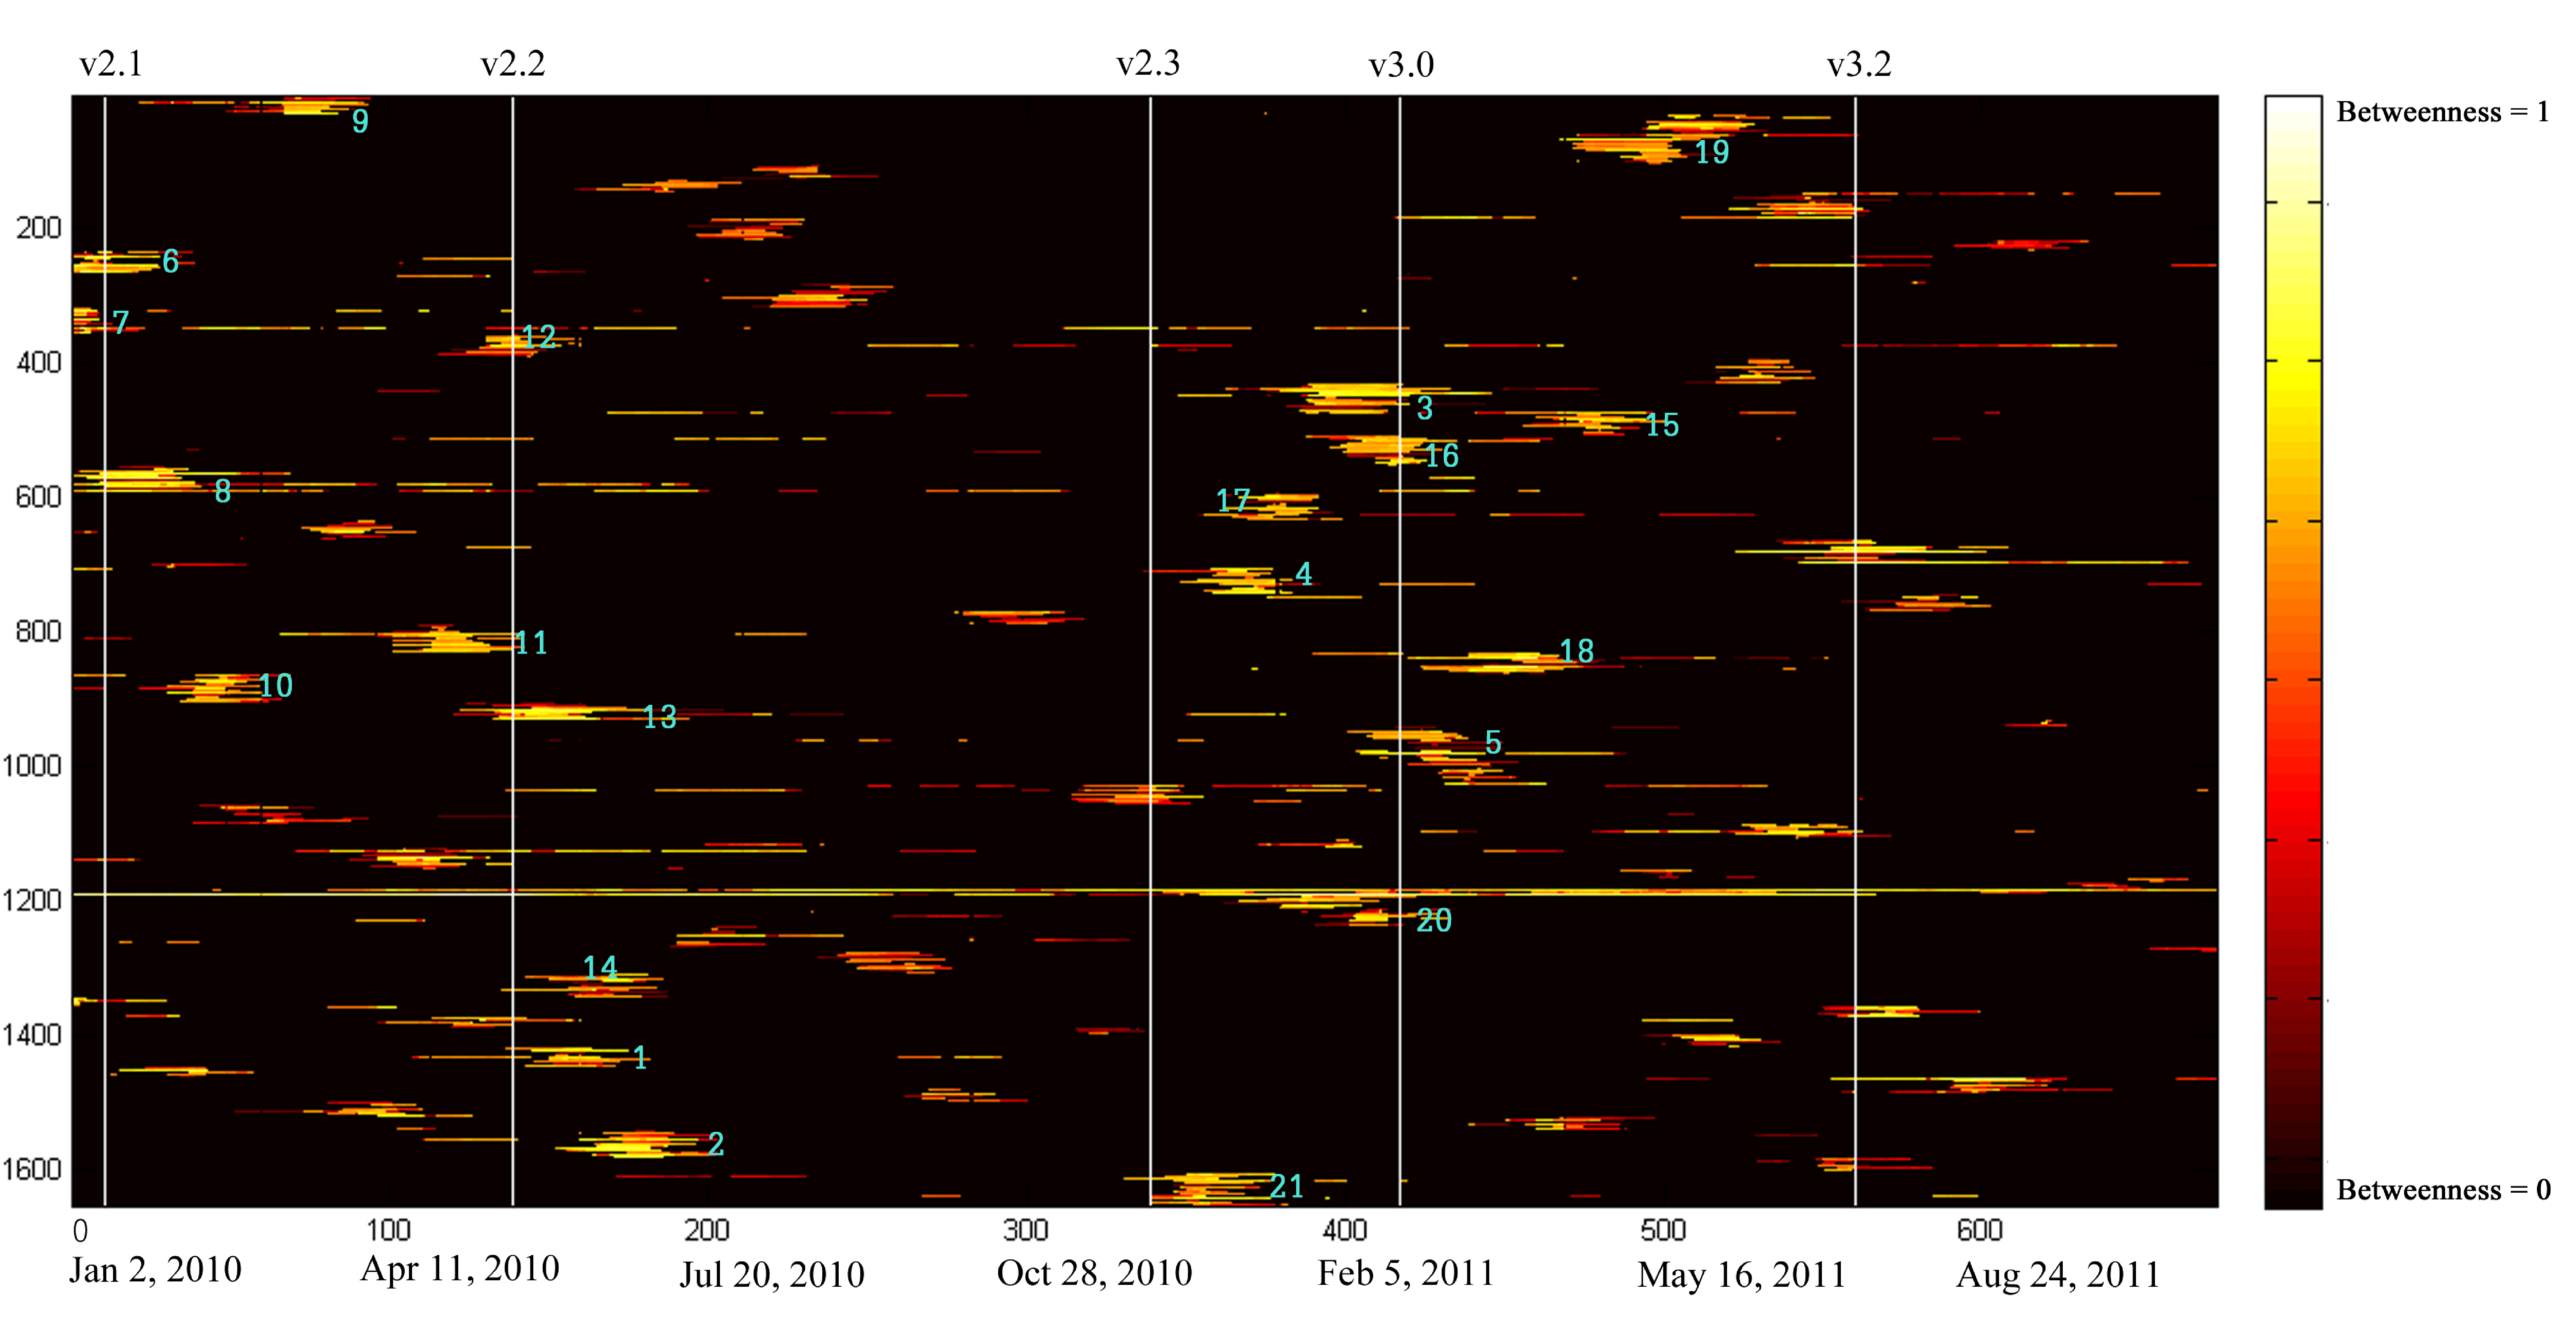
\includegraphics[width=18cm]{result.pdf}
\label{result}
\caption{Betweenness centrality along time line: the x-axis represents the
number of time windows and the starting dates are denoted every 100
windows. The y-axis represents the number of bug participants who have
ever been central in the bug community with betweenness
centrality valued greater than 0 for some time period. The
color represents the value of betweenness centrality, with darker
colors corresponding to lower betweenness and lighter colors for
higher betweenness. }
\end{figure*}


<<<<<<< HEAD

\subsection{Clustering}
Figure 3(1) orders participants by their betweenness values. We can indeed find that there are participants of low overall betweenness but being very active(show up bright) at some time points, and this supports the necessary of windowing, as stated in section \ref{overlappingtimewindowing}. However, we need more information about participants' working patterns and get an idea about their being interacting groups. 

In order to perceive clusters, that are local groups of interactions,
we clustered the bug participants using K-means by their betweenness centrality
distribution along the time line.  
K-means is one of the most popular
clustering methods which aims to partition n data items into $k$ clusters that each data item belongs to the cluster with the nearest mean \cite{MATH:macqueen}. 
We choose to use K-means with cosine distance.
The
cosine distance between two vectors is defined as,

\begin{equation}
cosine\_dist(A,B) = 1-\frac{A\cdot B}{\Arrowvert A \Arrowvert \Arrowvert B \Arrowvert}
\end{equation}

where A and B are two vectors, $\cdot$ represents the inner dot
operation and $\Arrowvert \cdot \Arrowvert$ indicates the module of
the vector. With clustering, authors with similar temporal centrality would be
grouped together so that bug participants with similar activity
patterns are also grouped together. 

In this paper, we choose the K-means with cosine distance because it gives a better clustering result, as compared in the plots of Figure 3(2) and Figure 2.
In this case, cosine distance calculates the similarity between each pair of
participants in terms of temporal centrality whereas Euclidean distance
focuses on the magnitude of data, the size and frequency of centrality.

Moreover, we used $k = 100$ for the K-means, to cluster authors. As we can see from Figure 3(3), k = 10 also gives good visualization result, but considering the number of more than 1600 participants, we should get a larger k to keep the diversity of working groups in similar. There is a trade off between the size of clusters and the variance within each cluster. We set $k = 100$ in this case, since we get the aesthetically best visualization (our
subjective opinion based on visible clusters) of all the data with 100
clusters. 

\section{Methodology}
\label{methodology}
\subsection{Data}

With the provided Android bug repository and the Android version
control system
from the MSR Challenge~\cite{DATA:msr}, we converted the XML format data and stored to
a database for efficient analysis using Microsoft SQL Server Business
Intelligence. Our analysis focused on the bug records of the previous
two years from January 1st 2010 to December 4th 2011 since during these two years, participants
are more active than the other years according to the records in the repository; also, the
activities are representative, both the Android platforms and their developer groups are larger and more diverse during the latest two years and it was also more relevant to modern Android handsets. The data we used of these two years 
covers 14,432 out of 20,169 total bug records and 46,806 out of 67,730
total bug comments from the whole dataset. Related to these bug and comment records, there
are 30,969 people who have either reported a bug or made comments on a
bug.


The bug and comment records are grouped into 30-day windows sliding by
1 day. 
%The strategy of taking 30 days as a window and sliding by 1 day
%would be discussed in detail in Section \ref{methodology}. 
We extracted 673 windows in total from the bug reports during year 2010 and 2011.

In addition, we made use of the data from the Android version control
system (git)
to validate the mining results.
%  The 
% ``project'' \ and the ``target'' \ schema record all the submitted files from
% the developers, from which the actual behaviours could be identified.



\subsection{Windowing Bug Reports and Extracting Social Networks Methodology}
We windowed the data based on the time series and constructed networks
that indicated the relations among the participants within each specific
time window. For each window, we calculated the betweenness centrality of each
participant and plotted the centrality per participant in a visualization. The steps of our methodology are
explained as following:


\textbf{Step 1: Pruning the data.} We pruned the records of the
reporters and commenters into a pure name format, which are originally
recorded in semi-anonymous email formats in the XML repository dump. 
For example, given the original email address which is represented by
\textquotedblleft mathias....@gmail.com\textquotedblright, we truncate
the string starting from \textquotedblleft ....\textquotedblright \
and keep the front part \textquotedblleft mathias\textquotedblright \
at the beginning as the name of the reporter or commenter. 
This strategy could lead to name aliasing problem, especially for
common names or email addresses starting at just a simple letter like
\textquotedblleft e....@gmail.com\textquotedblright.
 Although algorithms have been provided to reduce the extent of the problem, \cite{ACM:robles}, \cite{ACM:bird}, \cite{Elsevier:goeminne}, it is difficult or even impossible to eliminate the influence from
 this problem. Hence, we focus on the behaviour of normal cases, which
 means the cases where the names are less common and less ambiguous.


\textbf{Step 2: Windowing the records.} We windowed the data into
periods of 30 days with a 29-day overlap. 
30 days was chosen as a window size because it is smaller than the
periods between a major and minor release, it is similar to a month of
work, but long enough to contain the resolution of multiple bugs.
We have compared sliding by 1 day with our previous result of sliding by 7
days, 1 day sliding produces gradual and smoother transitions of
centrality.


\textbf{Step 3: Establishing the network.} We made a tool to perform the SNA with sliding
windows. The tool is implemented in Java and built on top of the JUNG Graph Framework, that converted bug
reports and bug comment records within a window to a social network graph.

The nodes of these networks represent participants who have either
reported some bugs or made comments on bugs. The edges represent
connections between two nodes. All the edges are weighted.  
For a bug within a selected time window, whenever a person
makes a comment on this bug, the edge between the bug commenter and
the bug reporter would get weight plus one, as well as the edges
linking to the participants who previously made comments on this
bug. Bug reports or comments in different windows would have separate
network graphs depending on the activity of their reporters or
commenters. An example in Figure 1 indicates how the weighted network
graph is built.


\textbf{Step 4: Calculating the centrality.} We calculated the
betweenness centrality using functionalities from JUNG, and normalized the centrality with the number of node pairs, as in Equation (\ref{normalizedb}). We then get a list of all the bug participants and
their betweenness centrality values for the total 673 overlapping
windows.


\textbf{Step 5: Removing irrelevant participants.} We removed the
participants with betweenness centrality value 0, who might have
either reported a bug/bugs with no comments, or made the only comment
on a bug so that no other participants are related. Afterwards, we get
1654 participants in total out of the 30969.


\textbf{Step 6: Generating the analysis graph.} The activity
of each bug participant is represented by a 673 dimensional vector. Each element of the vector indicates the betweenness centrality value extracted
from the graph, which is generated from the window for that
specific time period (in our case, the specific time period is 30 days
starting from the date of the window start point). Then we clustered
all the vectors by using K-means ($K=100$) with cosine distance to 100
clusters. Finally, we plotted the results, as shown in Figure 2 to
visualize the clustered data so that we could easily analyze
our results.


\subsection{Validating with the Android release history and the git.} 
In addition to the methodology of mining the Android
bug repository, we made use of the git and
inspected the release history to validate the purpose behind the
clusters we observed.
We looked into the participants who ever contributed to the git to find their areas of expertise and find out how the community participants
act in accordance with the project development.

The types of files modified and the corresponding projects are highly
correlated with the skills of those who commit changes. For
instance, if a developer always submits kernel related code
files, they are more likely to be specialized in kernel techniques. Types of files
include document files, test files, source files, etc; dictionary paths of files usually indicate what projects the files contribute to. 
We manually identified the participants' areas of expertise by
observing the ``project'' and the
``target'' for all of their commits (such as source code or
documentation).
To give a specific example, if there were commits from a developer,
Mr. Guilfoyle, on the file
media/java/android/media/Ringtone.java under the project
platform\_frameworks\_base; then, we would suggest that Mr. Guilfoyle 
likely has some specialized knowledge about the platform's ringtone. 
Thus this is how we derive participant expertise.

Also, we could further relate their expertise to their centrality
patterns. The Android release history could, on the other hand, help
to relate the release highlights to participants central behaviour during
that release. Further validation is discussed in Section
\ref{validation}. 


=======
\subsection{Windowing Bug Reports and Extracting Social Networks Methodology}
We windowed the data based on the time series and constructed networks
that indicated the relations among the participants within each specific
time window. Per each window, we calculated the betweenness centrality of each
participant and plotted the centrality per author in a visualization. The steps of our methodology are
explained as following:


\textbf{Step 1: Pruning the data.} We pruned the records of the
reporters and commenters into a pure name format, which are originally
recorded in semi-anonymous email formats in the XML repository dump. 
For example, given the original email address which is represented by
\textquotedblleft mathias....@gmail.com\textquotedblright, we truncate
the string starting from \textquotedblleft ....\textquotedblright \
and keep the front part \textquotedblleft mathias\textquotedblright \
at the beginning as the name of the reporter or commenter. 
This strategy could lead to name aliasing problem, especially for
common names or email addresses starting at just a simple letter like
\textquotedblleft e....@gmail.com\textquotedblright.
 It is difficult or even impossible to eliminate the influence from
 this problem. Hence, we focus on the behaviour of normal cases, which
 means the cases where the names are less common and less ambiguous.


\textbf{Step 2: Windowing the records.} We windowed the data into
periods of 30 days with a 29-day overlap. 
30 days was chosen as a window size because it is smaller than the
periods between a major and minor release, it is similar to a month of
work, but long enough to contain the resolution of multiple bugs.
We have compared sliding by 1 day with our previous result of sliding by 7
days, 1 day sliding produces gradual and smoother transitions of
centrality.


\textbf{Step 3: Establishing the network.} We made a SNA sliding
window tool with Java and the JUNG Graph Framework, that converted bug
reports and bug comment records within a window to a social network graph.

The nodes of these networks represent participants who have either
reported some bugs or made comments on bugs. The edges represent
connections between two nodes. All the edges are weighted.  
For a bug within a selected time window, whenever a person
makes a comment on this bug, the edge between the bug commenter and
the bug reporter would get weight plus one, as well as the edges
linking to the participants who previously make comments on this
bug. Bug reports or comments in different windows would have separate
network graphs depending on the activity of their reporters or
commenters. An example in Figure 1 indicates how the weighted network
graph is built.


\textbf{Step 4: Calculating the centrality.} We calculated the
betweenness centrality with JUNG, and normalized the centrality by
dividing by the number of node pairs excluding the current node
($(n-1)(n-2)/2$). We then get a list of all the bug participants and
their betweenness centrality values for the total 673 overlapping
windows.


\textbf{Step 5: Extracting the participants.} We removed the
participants with betweenness centrality value 0, who might have
either reported a bug/bugs with no comments, or made the only comment
of on a bug so that no other participants are related. Afterwards, we get
1654 participants in total out of the 30969.


\textbf{Step 6: Generating the analysis graph.} The activity
of each bug participant is represented by a 673 dimensional vector with
each element indicating the betweenness centrality value extracted
from the graph generated from the window for that
specific time period (in our case, the specific time period is 30 days
starting from the date of the window start point). Then we clustered
all the vectors by using K-means ($K=100$) with Cosine distance to 100
clusters. The reason for clustering into 100 clusters is that from
experiments, we get the aesthetically best visualization (our
subjective opinion based on visible clusters) of all the data with 100
clusters. Finally, we plotted the results, as shown in Figure 3 to
visualize the clustered data so that we could easily analyze
our results.


\textbf{Step 7: Validating with the Android release history and change
  repository.} In addition to the methodology of mining the Android
bug repository, we made use of the Android version control system
(git) and
inspected the release history to validate the purpose behind the
clusters we observed.
In order to find out how the community participants
act in accordance with the project development and why some
participants are more likely to be clustered into the same group, we
looked into their commit history to find their areas of expertise.


The types of files modified and the corresponding projects are highly
correlated with the skills of those who commit changes. For
instance, if a developer always submits kernel related code
files, they are more likely to be specialized in kernel techniques. We
extracted the submissions related to the developer from the version
control system.
We manually identified the participants areas of expertise by
observing the ``project'' and the
``target'' for all of their commits (such as source code or
documentation).
To give a specific example, if there were commits from a developer,
Mr. Guilfoyle, on the file
media/java/android/media/Ringtone.java under the project
platform\_frameworks\_base; then, we would suggest that Mr. Guilfoyle 
likely has some specialized knowledge about the platform's ringtone. 
Thus this is how we derive participant expertise.

Also, we could further relate their expertise to their centrality
patterns. The Android release history could, on the other hand, help
to relate the release highlights to participants central behaviour during
that release. Further validation is discussed in Section
\ref{validation}. 

>>>>>>> 788897dc7945851dec3c2974deb2851042e0fbd1

\begin{figure}[!t]
\centerline{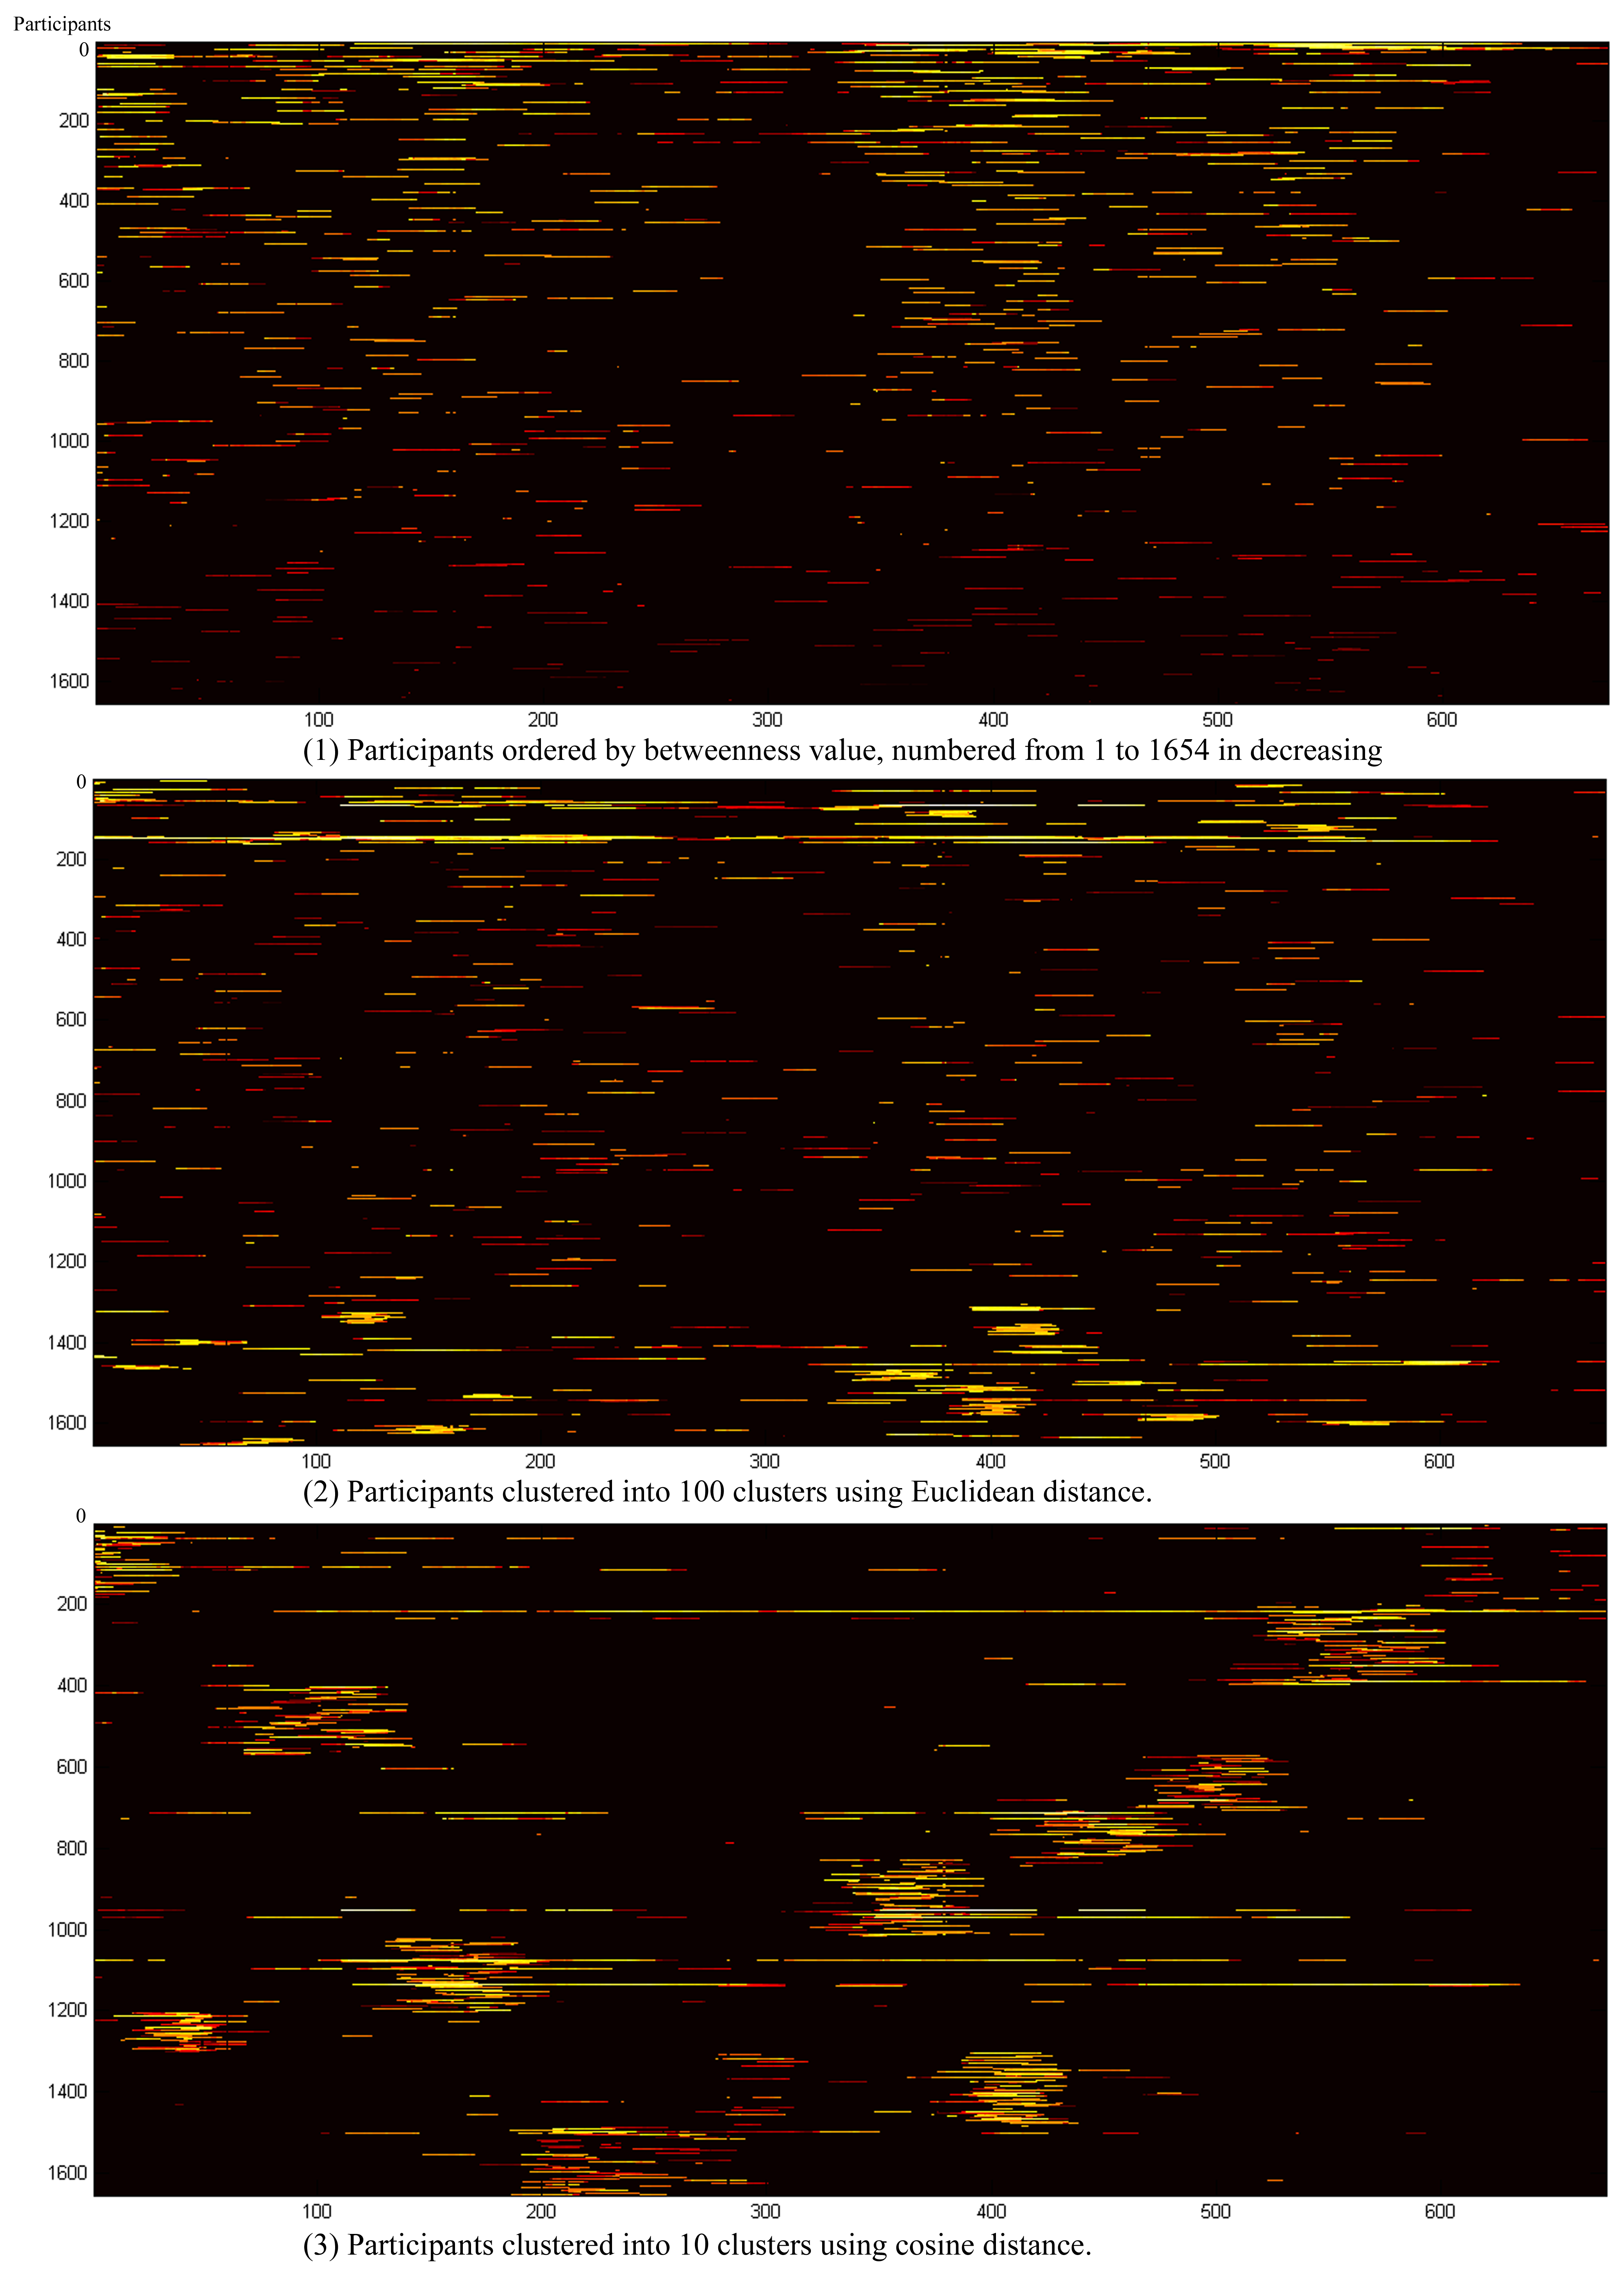
\includegraphics[width=3.54in]{cluster_comp.png}
\label{cluster_comp}}
\caption{Betweenness centrality along time line. Participants on the y-axes are ordered differently by betweenness values or various clusterings. }
\end{figure}

\section{Results and Analysis}
% describe the figure. 
% take up two columns
\label{results}
<<<<<<< HEAD

We study the results shown in Figure 2. Each horizontal line represents the 673 betweenness
centrality values for the selected bug participant during year 2010 and
2011. In total, we have 1654 bug participants. By studying these results, we answered the
following questions:


\subsection{Global Trends}

\textbf{RQ1. How does the number of active bug participants change over time? Why?}

To give an overview, we compared the interaction of bug participants
between January, 2010 and December, 2011, and found that the
interaction among participants in the Android bug community in 2011 was similar
to the interaction of participants in 2010 but more frequent, as we can also see in Figure 4 that the number of active participants
during 2011 is slightly larger than that of 2010. One
``gap'' occurs around window 300,
which we will explain in the next Local Comparison subsection. 

A possible reason for the changes of the number of active bug participants
and the betweenness centrality values is that around major or minor
releases of SDKs, API fixes or improvements, participants seem to become more
active in bug reporting, discussing and fixing
activities. Also, during these time periods, bugs are more likely to
be discovered and reported. 
Perhaps the pressure of the release is 
causing developers to address outstanding bugs more than usual.
% AH: You can't just say this stuff, if you don't know you gotta admit it
% would probably work longer and harder than usual with more
%effort and passion, which promotes the discovery of more bugs and
%problems of the project. 
%And when the release date is approaching,
%they have to work hard to fix these bugs. 
After a
release, users also take part in the activity of
discovering the bugs and problems so that in this case both users and
developers would like to discuss the bugs. 
%The bug community becomes
%lively. 


\textbf{RQ2. How does the betweenness centrality of a participant change over time? What are the reasons when they have a certain activity pattern?}

Observing the continuity of betweenness centrality in Figure 2, some
participants have kept active during the entire two years, and
correspondingly they have a very continuous and bright line. For
participants of this type, there are a few possible explanations. 

% XXX IN THE PRESENTATION YOU NAMED NAMES. STOP GUESSING. TELL US IF
% THIS IS THE CASE
First, our conjecture is that these participants are professional developers who
belong to the core development team so that what they reported are
more important issues which attract more participants to discuss and fix
them. 
% XXX VERIFY THIS SENTENCE IS IT TRUE OR NOT?
When investigating some of the continuous lines we found some
participants were Google employees, for example, two developers with alias mbligh and romainguy.
Their email account recorded in the git are under the \textquotedblleft google.com\textquotedblright \ domain, and moreover, when we googled them, they are indeed introduced as software engineers at Google. 

% XXX YOU SAID THIS IN THE PRESENTATION AND HAD EXAMPLES DID YOU LOOK
% AT THIS OR NOT
Second, some of these participants are of high community status or
expertise, and they might
supervise and guide the development of the 
project. When we validated, we did find one developer, romainguy, who has experiences on almost every component relevant to platforms so that he can be considered to be an expert.
%They would like to report big issues and will give expert
%comments on bugs. 
% XXX PLEASE GIVE AN EXAMPLE WHERE DID THE VALIDATION GO

Developers related to these continuous lines are listed in Table \ref{continuous_project}, and we will further discuss and validate on them in Section \ref{validation}.

However, in most cases, participants' betweenness values are
highly variant, as observed in Figure 2. 
To investigate the variation in betweenness values over time, we
decided to count the number of times that a user experienced a range of consecutive windows in
which the user had non-zero betweenness.
% We counted the
% number of occurrences of the continuous betweenness values which are
% greater than 0. 
% It means that we would count 1 if the betweenness
% value is greater than 0 for the first time and take the next values
% together as the first continuous occurrence until we meet 0. 
% Then the
% second time we meet value greater than 0, we would count 2 and take
% the next values together as the second continuous occurrence until
% another 0 occurs. 
Participants who only had 1
distinct range of betweenness are considered to be participants who
only appeared once, and are probably users (validated in Section \ref{validation}). 
Participants with a count of distinct ranges
 greater than 1 would be phasers who periodically participate within
 the Android bug
community. Here phasers are those who
phase into centrality and later out of it.
These randomly phasing participants (\emph{phasers}) are very likely to
acquire less knowledge or have lower community status in their
community, than those with continuous high centrality. 
Phasers
might be interested in limited topics and only central and active
during the appearance of bugs relevant to those topics.
We validate the roles these participants play in Section \ref{validation}.

\subsection{Local Comparison}
\label{local}

\textbf{RQ3. Are there special time ranges during which participants are more/less active or central than normal? Why?}

By manually inspecting Android version history, we found that the v2.1
SDK was released on 12 January 2010, which corresponds to the first peak
value in Figure 5. Android v2.2 SDK was released on 20 May 2010 and this
corresponds to peak 2. From Dec. 2010 to the beginning of Mar. 2011,
several minor updates were released and on 22 Feb. 2011, one major
update v3.0 SDK was released. These releases explain the summit, i.e.,
peak 3, in  Figure 5. This is correlated with more participation at
the same time.

In addition, for the first obvious ``gap'', which covers the time from
October 2010 to the end of 2010 (around window 300), there were fewer
releases. The social network during this time period is almost inactive
and even ``quiet''.
=======

We study the results shown in Figure 2. The x-axis represents the
number of time windows and the starting dates are denoted every 100
windows. The y-axis represents the number of bug participants who have
ever been central in the bug community so that their betweenness
centrality values would be greater than 0 for some time period. The
color represents the value of betweenness centrality, with darker
colors corresponding to lower betweenness and lighter colors for
higher betweenness. Each horizontal line represents the 673 betweenness
centrality values for some bug participant during year 2010 and
2011. In total, we have 1654 bug participants. We clustered the data
using K-means with Cosine distance and numbered the participants from
1 to 1654. By studying these results, we answered the
following questions:


\subsection{Global Trends}

\textbf{RQ1. How does the number of active bug participants change over time? Why?}

To give an overview, we compared the interaction of bug participants
between January, 2010 and December, 2011, and found that the
interaction among participants in Android bug community in 2011 was similar
to the interaction of participants in 2010 but more frequent. One
``gap'' occurs around window 300,
which we will explain in the Section \ref{local} later. 


In Figure 4 the number of active participants
during 2011 is slightly larger than that of 2010. Also, we can observe
a ``gap'' around the window
300. Figure 5 shows the sum of betweenness values along the two years'
time line, we can see that the trend is very similar to that of the
number of active participants in Figure 4. This suggests that with more
participants participating in bug reporting community, the interaction among
them increases accordingly.


A possible reason for the changes of the number of active bug participants
and the betweenness centrality values is that around major or minor
releases of SDKs, API fixes or improvements, participants seem to become more
active in bug reporting, discussing and fixing
activities. Also, during these time periods, bugs are more likely to
be discovered and reported. 
Perhaps the pressure of the release is 
causing developers to address outstanding bugs more than usual.
% AH: You can't just say this stuff, if you don't know you gotta admit it
% would probably work longer and harder than usual with more
%effort and passion, which promotes the discovery of more bugs and
%problems of the project. 
%And when the release date is approaching,
%they have to work hard to fix these bugs. 
After a
release, users also take part in the activity of
discovering the bugs and problems so that in this case both users and
developers would like to discuss the bugs. 
%The bug community becomes
%lively. 


\textbf{RQ2. How does the betweenness centrality of a participant change over time? What are the reasons if they have a certain activity pattern?}

Observing the continuity of betweenness centrality in Figure 3, some
participants have kept active during the entire two years, and
correspondingly they have a very continuous and bright line. For
participants of this type, there are a few possible explanations. 

% XXX IN THE PRESENTATION YOU NAMED NAMES. STOP GUESSING. TELL US IF
% THIS IS THE CASE
First, we suspect these participants are professional developers who
belong to the core development team so that what they reported are
more important issues which attract more participants to discuss and fix
them. 
% XXX VERIFY THIS SENTENCE IS IT TRUE OR NOT?
When investigating some of the continuous lines we found some
participants were Google employees.

% XXX YOU SAID THIS IN THE PRESENTATION AND HAD EXAMPLES DID YOU LOOK
% AT THIS OR NOT
Second, some of these participants are of high community status or
expertise, and they might
supervise and guide the development of the 
project. 
%They would like to report big issues and will give expert
%comments on bugs. 
% XXX PLEASE GIVE AN EXAMPLE WHERE DID THE VALIDATION GO


However, in most cases, participants' betweenness values are
highly variant, as observed in Figure 3. 
To investigate the variation in betweenness values over time we
decided to count the number of times that a user experienced one or more
consecutive windows of betweenness, that is a range of windows in
which the user had non-zero betweenness.
% We counted the
% number of occurrences of the continuous betweenness values which are
% greater than 0. 
% It means that we would count 1 if the betweenness
% value is greater than 0 for the first time and take the next values
% together as the first continuous occurrence until we meet 0. 
% Then the
% second time we meet value greater than 0, we would count 2 and take
% the next values together as the second continuous occurrence until
% another 0 occurs. 
Participants who had less than a few windows of betweeness only had 1
distinct range of betweenness are considered to be participants who
only appeared once, and are probably users (validated in Section \ref{validation}). 
Participants with a count of distinct ranges
 greater than 1 would be phasers who periodically participate within
 the Android bug
community. 
These randomly phasing participants (\emph{phasers}) are very likely to
acquire less knowledge or have lower community status in their
community, than those with continuous high centrality. 
Phasers
might be interested in limited topics and only central and active
during the appearance of bugs relevant to those topics.
We validate the roles these participants play in Section \ref{validation}.
>>>>>>> 788897dc7945851dec3c2974deb2851042e0fbd1


The other low value showing up in the end of Figure 5 results from
the fact that there are no bug reports recorded (right tail censoring) in the given dataset.
This piece of data is still meaningful because it contains comments belonging to bug reports several weeks or months before. The betweenness value is thus simply calculated by the comments here. 

<<<<<<< HEAD

\textbf{RQ4. What are the possible scenarios for a very sharp change of the participants' centrality? Why?}

Considering individual participants, almost all of them has
experienced centrality oscillations. In addition, some participants
tend to become active and core members during the same time
period and then they fade away together.
=======
By manually inspecting Android version history, we found that the v2.1
SDK was released on 12 January 2010, which corresponds to the first peak
value in Figure 5. Android v2.2 SDK was released on 20 May 2010 and this
corresponds to peak 2. From Dec. 2010 to the beginning of Mar. 2011,
several minor updates were released and on 22 Feb. 2011, one major
update v3.0 SDK was released. These releases explain the summit, i.e.,
peak 3, in  Figure 5. This is correlated with more participation at
the same time.

In addition, for the first obvious ``gap'', which covers the time from
October 2010 to the end of 2010 (around window 300), there were fewer
releases. The social network during this time period is almost inactive
and even ``quiet''.


The other bottom value showing up in the end of Figure 5 results from
the fact that there are no bug reports recorded (right tail censoring) in the given dataset
and the betweenness value is simply calculated by the comments
belonging to bug reports several weeks or months before. 

>>>>>>> 788897dc7945851dec3c2974deb2851042e0fbd1


<<<<<<< HEAD
We suspect that the phasers tend to be interested in one or several
categories of problems so that they appear only along with the
occurrence of these issues. They take part in activities related to
the bugs or technical issues and become inactive after the problems are
solved. Or in the case when they are working on a project, they would become inactive when the projects are finished. 
As showed in Figure 2, the participants' tend to get clustered together around important releases, which supports that the phasers are working along with projects or related issues.
Meanwhile, by observing the clustered participants of their
activity patterns in Figure 2, we suspect that the phasers that show
up densely together could be interested in similar categories of
topics. 
This assumption is validated in Section
=======
Considering individual participants, almost all of them has
experienced centrality oscillations. In addition, some participants
tend to become active and core members during the same time
period and then they fade away together. We call them phasers, who
phase into centrality and later out of it.


We suspect that the phasers tend to be interested in one or several
categories of problems so that they occur only along with the
occurrence of these issues. They take part in activities related to
the bugs or technical issues and become inactive after the problems
solved. Also, by observing the clustered participants of their
activity patterns in Figure 3, we suspect that the phasers that show
up densely together could be interested in similar categories of
topics. This assumption is validated in Section
>>>>>>> 788897dc7945851dec3c2974deb2851042e0fbd1
\ref{validation}. 


\begin{figure}[!t]
\centerline{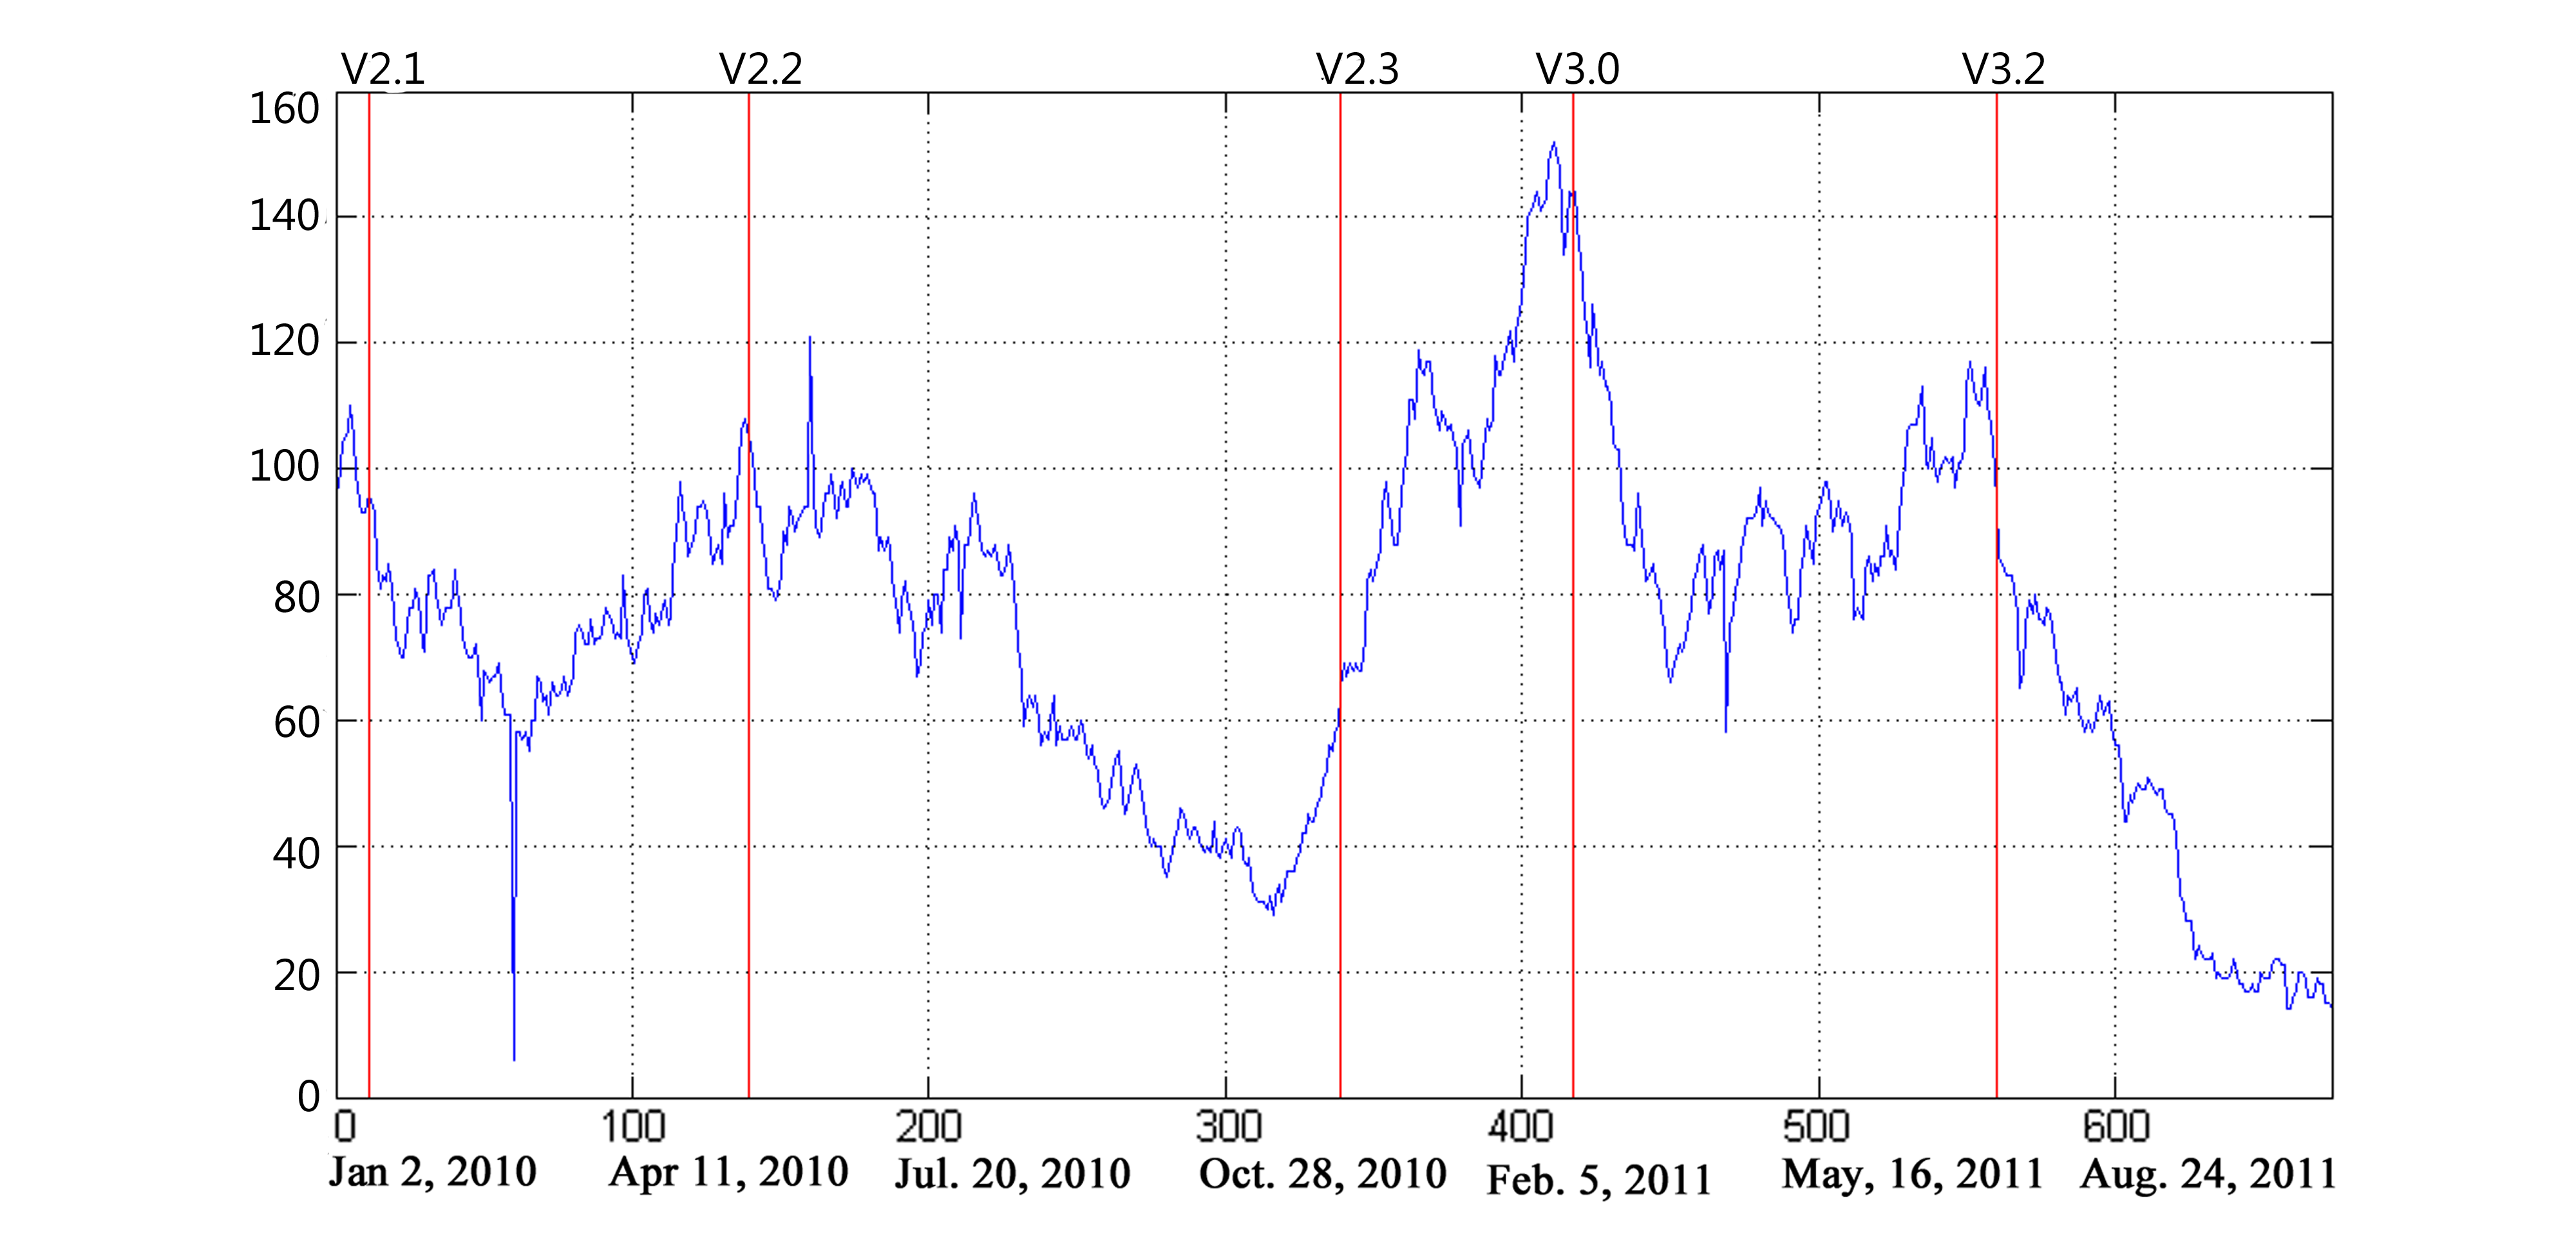
\includegraphics[width=4.1in, height = 3.8cm]{people.png}
\label{people}}
\caption{Number of active participants across time.}
\end{figure}

\begin{figure}[!t]
\centerline{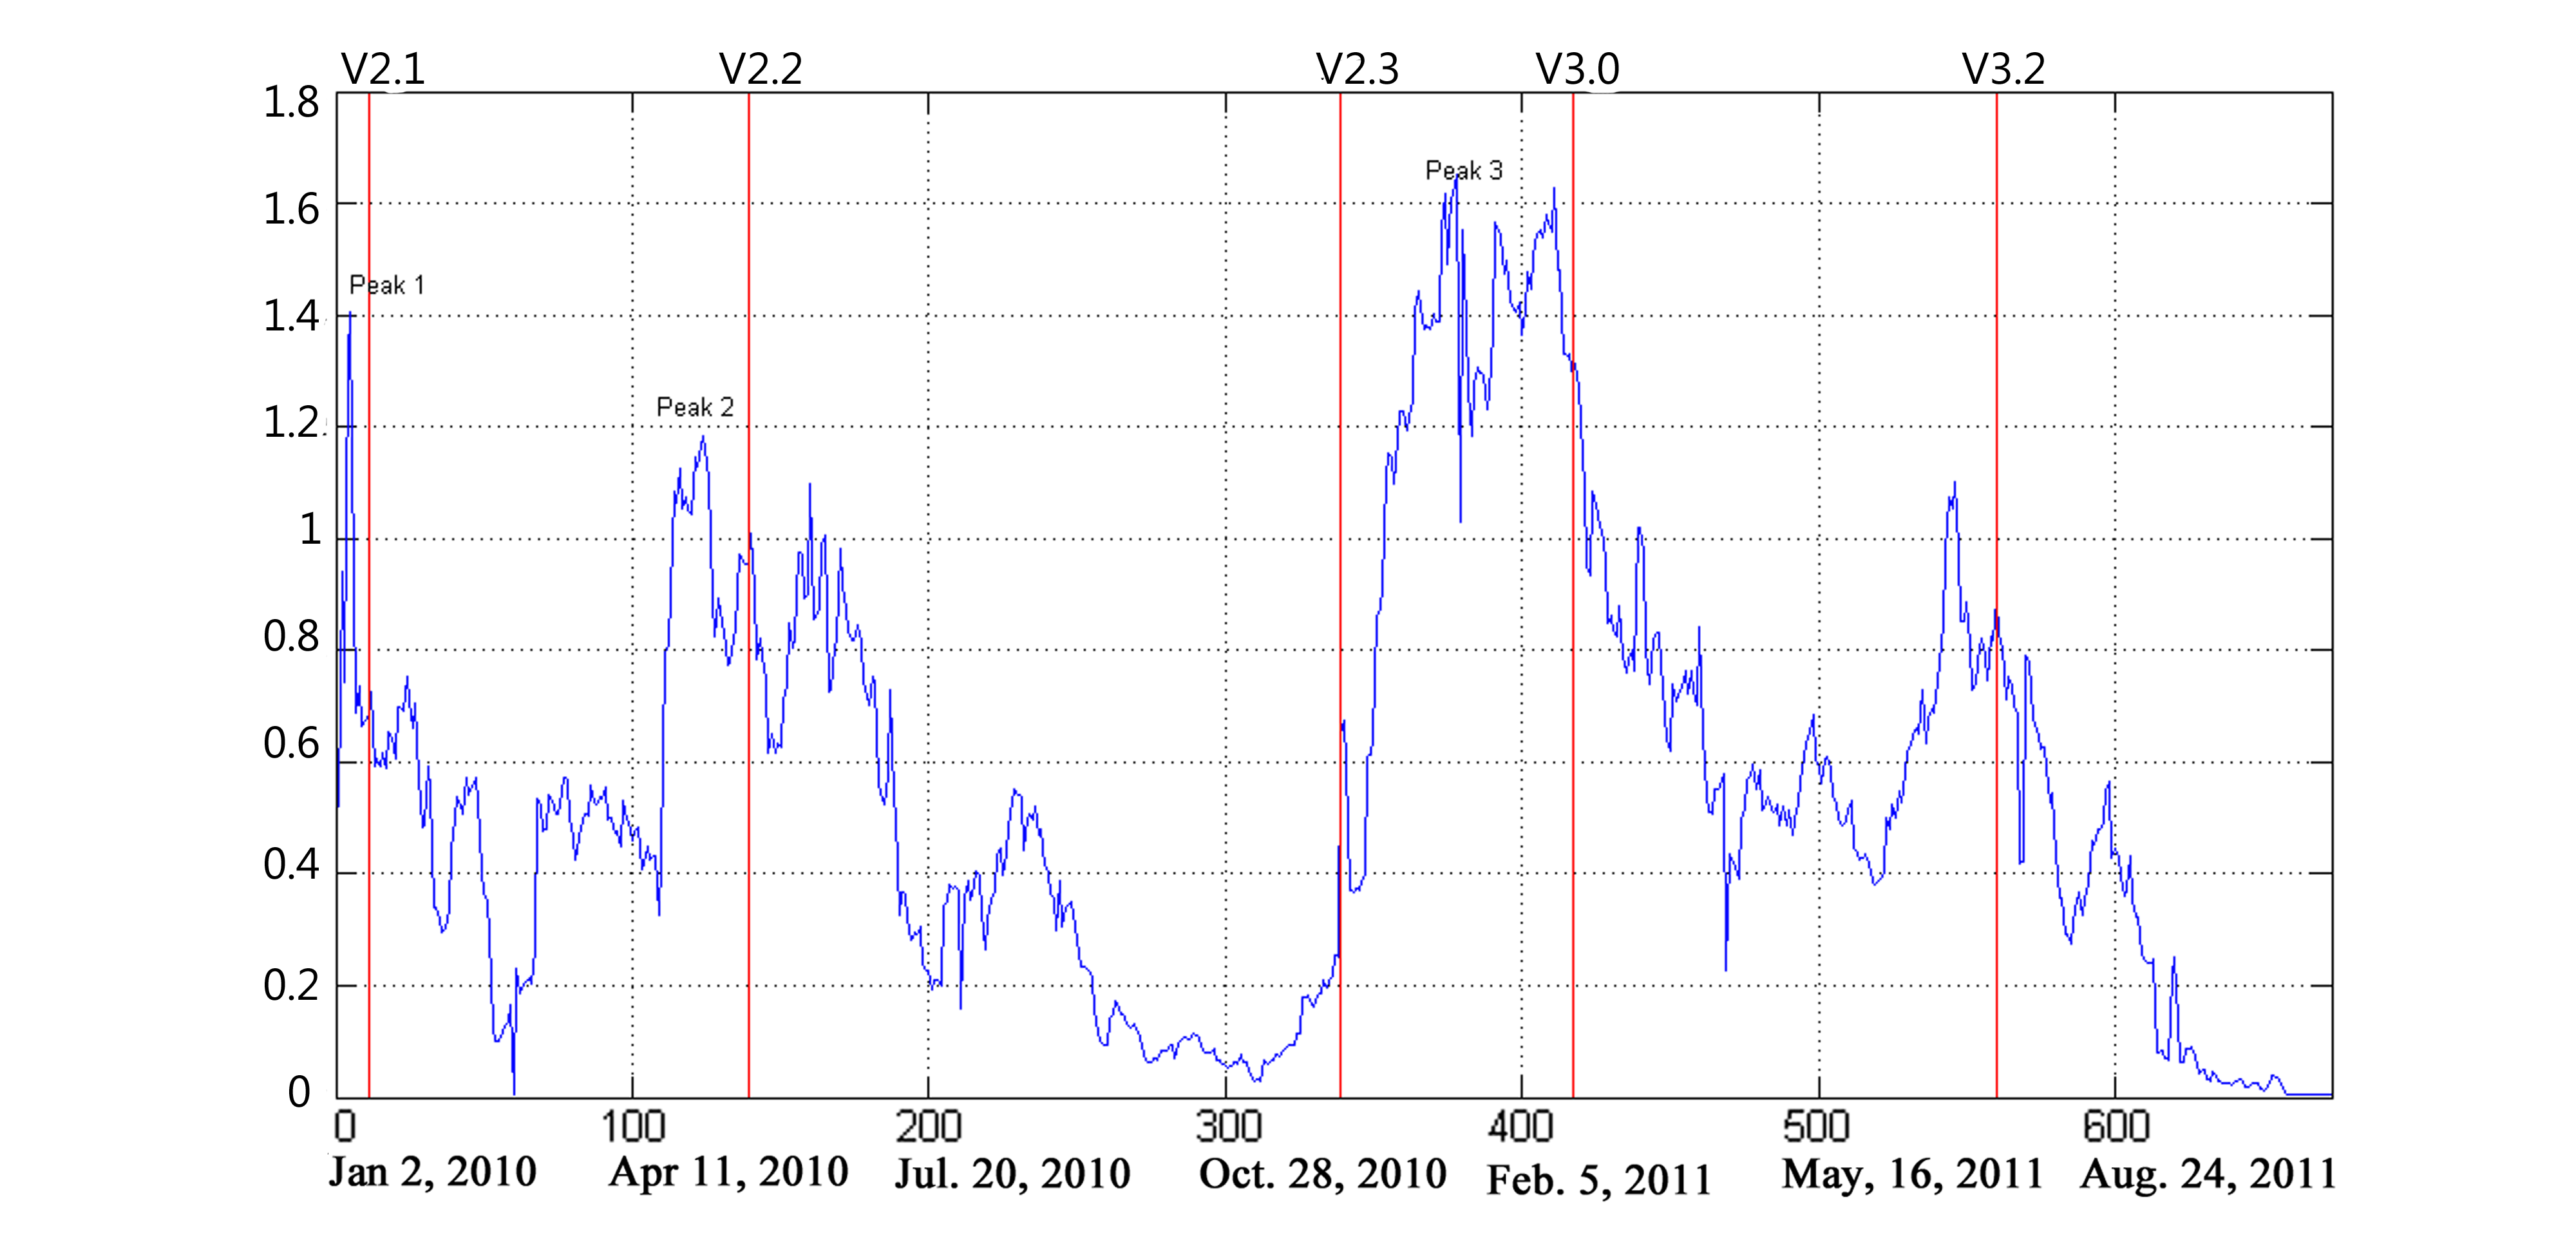
\includegraphics[width=4.1in, height = 3.8cm]{betweenness.png}
\label{betweenness}}
\caption{Sum of betweenness centrality of participants across time.}
\end{figure}

%XXX again you don't answer a research question by making stuff up
% relate this to your validation or remove it.
% If it can't be validated don't bother saying it as an answer to a question.
<<<<<<< HEAD
%Meanwhile, other possible explanations for the very sharp change in
%the participants' centrality could be: 1) the participants are pure
%users; they showed up merely to report bugs they found. These bugs
%attract other users or developers to take part in the discussion,
%which would increase the betweenness centrality of the bug reporters,
%i.e., the users, for a very short time period. 2) The participants are
%developers and are on a temporary leave, a vacation for
%example. 
%3) The project is just
%finished or discarded so that both users and developers would not
%discuss anything about it any more. This group of participants could be
%verified by looking for those who do not own any submission and then
%regarded as pure users. 
%The third explanation would be easily
%substantiated by inspecting Android version release history. However,
%the second explanation is hard or even impossible to validate with the
%very limited information we could get from the repositories and the
%release history. Participants should be contacted in person for such
%validation, which has not been done in our study.
=======
Meanwhile, other possible explanations for the very sharp change in
the participants' centrality could be: 1) the participants are pure
users; they showed up merely to report bugs they found. These bugs
attract other users or developers to take part in the discussion,
which would increase the betweenness centrality of the bug reporters,
i.e., the users, for a very short time period. 2) The participants are
developers and are on a temporary leave, a vacation for
example. 
3) The project is just
finished or discarded so that both users and developers would not
discuss anything about it any more. This group of participants could be
verified by looking for those who do not own any submission and then
regarded as pure users. 
The third explanation would be easily
substantiated by inspecting Android version release history. However,
the second explanation is hard or even impossible to validate with the
very limited information we could get from the repositories and the
release history. Participants should be contacted in person for such
validation, which has not been done in our study.
>>>>>>> 788897dc7945851dec3c2974deb2851042e0fbd1
%XXX GRRR Answer the question! Stop making stuff up. Link it to evidence.



%XXX This section needs to be integrated with the research question
%answers. I don't have the time to do this. 

\section{Validation}
\label{validation}
% This section needs to be modified!!!
% two parts: 1. assumption, take up 2 columns 2. validation, take up 3 columns
% validation: 1. clusters 2. phasers
We made use of the git and inspected the
release history to validate our answers to the research questions in the previous section.
For RQ1, it could only get answered based on assumption but not validated. RQ3 is intuitively answered when we match the betweenness distribution with the release history by time, and no further validation is needed. For RQ 2 and RQ4, we have made a detailed validation in this section.

\subsection{Activity pattern validation}

Among the 1654 participants with betweenness values larger than 0, we
analyzed their centrality patterns and divide them into three
categories: 
<<<<<<< HEAD

1) participants appeared only once with a betweeness greater than 0 (71 out of 1654
participants),
2) participants recurred periodically (1575 participants)
and 3) participants who are central along during the entire project
history (8 participants).


From the mining results, we notice that there is a small group of
participants who have been central for most of our analysis period; another
relatively larger group appear without any recurrence; the majority
would periodically become central in their community. Based on the
three activity patterns, we confirmed many of our previous suspicions:

%XXX MENTION WHICH RQ IS RELEVANT
\subsubsection{Participants that appeared only once tend to be pure users}

We look into the git to find the files
submitted by the 71 participants who have appeared only once in the
bug community. We found that only 7 of them have ever submitted a
=======

1) participants appeared only once with a betweeness greater than 0 (71 out of 1654
participants),
2) participants recurred periodically (1575 participants)
and 3) participants who are central along during the entire project
history (8 participants).


From the mining results, we notice that there is a small group of
participants who have been central for most of our analysis period; another
relatively larger group appear without any recurrence; the majority
would periodically become central in their community. Based on the
three activity patterns, we confirmed many of our previous suspicions:

%XXX MENTION WHICH RQ IS RELEVANT
\subsubsection{Participants appeared only once tend to be pure users}

We look into the Android version control system to find the files
submitted by the 71 participants who have appeared only once in the
bug community. We find that only 7 of them have ever submitted a
>>>>>>> 788897dc7945851dec3c2974deb2851042e0fbd1
change, which means that these 7 probably are likely developers rather
than pure Android users. The rest do not have commits in the version
control system. This verifies our assumption that participants
appeared only once in the bug community would more likely be pure
<<<<<<< HEAD
users, as introduced in RQ2.
=======
users.
>>>>>>> 788897dc7945851dec3c2974deb2851042e0fbd1

%XXX MENTION WHICH RQ IS RELEVANT
\subsubsection{Participants showed up periodically should be a combination of users and developers}
% y=742-704 + 1
% x=474 - 430 + 1
% z = 1447 - 1418 + 1
% y = 1584 - 1543 + 1
% u = 1584 - 1543 + 1
% y=742-704 + 1
% y
% 39
% u
% 42
% u+y+x+z
% 156
% (5+13+9+7)/(u+y+x+z)
% .21794871794871794871

Periodically appearing participants are the majority and we call them
\emph{phasers}. 
% We sampled 4 continuous portions of them (continuous
% means they are continuously numbered in the clustered results):
% participants 430 to 474, 704 to 742, 1418 to 1447, and 1543 to
% 1584. For each of the four groups, the number of developers are 5, 13,
% 9, 7 respectively. They take up 17\%, 32\%, 20\%, and 18\% of the
% total number of participants in each group. 
<<<<<<< HEAD
As the approach described in section \ref{methodology}, looking into the git to manually recognize a participant's expertise takes efforts; with as many as 1575 participants, we sampled 156 participants. $21.8\%$ of the sampled participants were developer phasers, who have ever submitted changes.
=======
We sampled 156 participants and of them $21.8\%$ were developer phasers.
>>>>>>> 788897dc7945851dec3c2974deb2851042e0fbd1

We studied the expertise of the developer participants from this
sample. All except two of them have worked on single focus tasks that
implied some kind of expertise or specialization.

<<<<<<< HEAD
The rest $78.2\%$ have never
submitted files to the development community. They are probably users
of Android. Thus, phasers consist of both users and
developers. This answers to our assumption of the phasers' role in RQ2.
=======
The rest of the periodically appearing participants have never
submitted files to the development community. They are probably users
of Android. Thus, phasers consist of both users and
developers. Developers of this group are tended to focus on specific
topics.
>>>>>>> 788897dc7945851dec3c2974deb2851042e0fbd1



\begin{table}[!t]
%% increase table row spacing, adjust to taste
% if using array.sty, it might be a good idea to tweak the value of
% \extrarowheight as needed to properly center the text within the cells
<<<<<<< HEAD
\caption{5 continuously central participants who have submitted changes to the git. On the forth row, ralf and Ralf.Hildebrandt are email alias of the same person, as we observed that the author\_name attributes are the same for the two email alias.}
=======
\caption{5 continuously central participants who have submissions in the version control system. On the forth row, ralf and Ralf.Hildebrandt are email alias of the same person, as we observed that the author\_name attributes are the same for the two email alias.}
>>>>>>> 788897dc7945851dec3c2974deb2851042e0fbd1
\label{continuous_project}
\centering
%% Some packages, such as MDW tools, offer better commands for making tables
%% than the plain LaTeX2e tabular which is used here.
\begin{tabular}{|p{1.2cm}|p{1.1cm}|p{4.6cm}|}
\hline
Participant & \#Submitted-\_changes & Related Project \\
\hline
fadden & 1259 & device\_samsung\_crespo, platform(bionic, build, dalvik, etc.) \\
\hline
xav & 3501 & platform(frameworks\_base, build, external\_bouncycastle, etc.), device\_sample, \\
\hline
mbligh & 80 & kernel(common, experimental, linux-2.6, msm, omap, qemu, samsung, tegra) \\
\hline
ralf (Ralf.-Hildebrandt) & 665 & kernel(common, experimental, linux-2.6, dalvik, external\_libpng, sdk,system\_core, etc.) \\
\hline
romainguy & 1455 & device\_htc\_passion, device\_samsung\_crespo, platform(build, cts, dalvik, development, external\_bouncycastle, libcore, ndk, apps(AccountsAndSyncSettings, AlarmClock,
Bluetooth, Browser, Calculator, etc.),
inputmethods(LatinIME, iOpenWnn, PinyinIME, CalendarProvider),
providers(DownloadProvider, GoogleSubscribedFeedsProvider), wallpapers(Basic, LivePicker,
MagicSmoke, MusicVisualization), prebuilt, sdk, system\_core) \\
\hline
\end{tabular}
\end{table}

%XXX MENTION WHICH RQ IS RELEVANT

<<<<<<< HEAD
\subsubsection{Participants who were continuously central for a long time period could have multiple areas of expertise}

5 out of the 8 participants in this group have submissions in the
git.
=======
\subsubsection{Participants who were continuously central could have multiple areas of expertise}

5 out of the 8 participants in this group have submissions in the
version control system.
>>>>>>> 788897dc7945851dec3c2974deb2851042e0fbd1
% XXX What did you mean here VVV this makes no sense whatosever
% and they take up to 62.5\%, which is significantly
% larger than the previous two groups.
We extracted the projects these 5 participants have submitted changes
to, as listed in Table \ref{continuous_project}.
<<<<<<< HEAD


Firstly, considering the number of changes they made, all of them
except \texttt{mbligh} have more than 500 commits within the
git,
which means that they are quite active in Android
development community. This supports that they are
experts or advanced developers since more submissions indicates a
 broader range knowledge about the related techniques.
% If you don't know, don't say it
%, especially
%in such volunteered open source development community.


Moreover, \texttt{fadden}, \texttt{xav}, and \texttt{romainguy} are
all working on the platform layer,
which includes build, dalvik, development, framework base, libcore,
sdk, etc. All of their areas of expertise are related to the platform layer or
system core layer.
% and should be important along the entire
%development. 
%In this case, continuously central participants should
%have experiences on the system core related topics. 
%This is an
%interesting point beyond our hypothesis.

The participant \texttt{romainguy} has experiences modifying almost every
component relevant to platforms, including both the apps and the core, and
hence should be considered as Android platform development leader.


To summarize, this subsection and the past 2 subsection demonstrate
that three different centrality patterns correspond to
participants of three categories, which supports our analysis hypothesis
in Section \ref{results}.

=======


Firstly, considering the number of changes they made, all of them
except \texttt{mblign} have more than 500 commits within the
version control system,
which means that they are quite active in Android
development community. This could to some extent prove that they are
experts or advanced developers since more submissions indicates a
 broader range knowledge about the related techniques.
% If you don't know, don't say it
%, especially
%in such volunteered open source development community.


Moreover, \texttt{fadden}, \texttt{xav}, and \texttt{romainguy} are
all working on the platform layer,
which includes build, dalvik, development, framework base, libcore,
sdk, etc. All of their areas of expertise are related to the platform layer or
system core layer.
% and should be important along the entire
%development. 
%In this case, continuously central participants should
%have experiences on the system core related topics. 
%This is an
%interesting point beyond our hypothesis.

The participant \texttt{romainguy} has experiences modifying almost every
component relevant to platforms, including both the apps and the core, and
hence should be considered as Android platform development leader.


To summarize, this subsection and the past 2 subsection demonstrate
that three different centrality patterns correspond to
participants of three categories, which proves our analysis hypothesis
in Section \ref{results}.

>>>>>>> 788897dc7945851dec3c2974deb2851042e0fbd1

\begin{table}[!t]
\centering
\caption{5 clusters we have chosen, out of a total number of 21.}
\begin{tabular}{|c|c|}
\hline
Cluster & Time  \\
\hline
1 & May 16, 2010 - Jun. 24, 2010 \\
\hline
2 & Jun. 2, 2010 - Jul. 24, 2010  \\
\hline
3 & Jan. 13, 2011 - Mar. 3, 2011 \\
\hline
4 & Dec. 3, 2010 - Jan. 31, 2010 \\
\hline
5 & Feb. 4, 2011 - May 1, 2011 \\
\hline
\end{tabular}
\label{cluster_list}
\end{table}

\begin{table}[!t]
%% increase table row spacing, adjust to taste
\renewcommand{\arraystretch}{1.3}
% if using array.sty, it might be a good idea to tweak the value of
% \extrarowheight as needed to properly center the text within the cells
\caption{Participants and their areas of expertise in cluster No. 4}
\label{cluster_no4}
\centering
%% Some packages, such as MDW tools, offer better commands for making tables
%% than the plain LaTeX2e tabular which is used here.
\begin{tabular}{|c|c|c|}
\hline
ID & Name & Areas Of Expertise \\
\hline
1 & charles & kernel - sound, kernel\_linux-2.6 \\
\hline
2 & jasta00 & ringtone, media \\
\hline
3 & kristoff & driver(net, video, serial, input) \\
\hline
4 & rik(rik.bobbaers) & kernel\_linux-2.6(mlock) \\
\hline
5 & rik(rikard.p.olsson) & kernel\_linux-2.6(arm) \\
\hline
6 & rik(riku.voipio) & kernel\_linux-2.6(arm), driver \\
\hline
7 & snp & platform sdk(eclipse plugin) \\
\hline
\end{tabular}
\end{table}

\begin{table*}[!t]
%% increase table row spacing, adjust to taste
% if using array.sty, it might be a good idea to tweak the value of
% \extrarowheight as needed to properly center the text within the cells
<<<<<<< HEAD
\caption{Participants' common areas of expertise of each cluster. Participants number is counted as the number of participants within each cluster who has ever submitted a change and appeared in the git, ie., developers.}
=======
\caption{Participants' common areas of expertise of each cluster. Participants number is counted as the number of participants within each cluster who has ever submitted a change and appeared in the change repository, ie., developers.}
>>>>>>> 788897dc7945851dec3c2974deb2851042e0fbd1
\label{cluster_topic}
\centering
%% Some packages, such as MDW tools, offer better commands for making tables
%% than the plain LaTeX2e tabular which is used here.
\begin{tabular}{|c|c|c|}
\hline
Cluster & Participants Number & Areas Of Expertise \\
\hline
1 & 5 & netfilter, driver(video), tests, MIPS \\
\hline
2 & 13 & driver(usb, wireless, mouse), sound, net, i386, performance(tools), input methods \\
\hline
3 & 9 & sound, driver, frameworks\_base, tests, platform, kernel \\
\hline
4 & 7 & sound, media, kernel\_linux-2.6, driver, platform sdk, kernel video/serial \\
\hline
5 & 63 & net(bluethooth, net driver, ipv$x$, kernel\_linux-2.6), driver(dvd, media, usb, gpu, net), ia64, sound, tests \\
\hline
\end{tabular}
\end{table*}

\begin{table*}[!t]
%% increase table row spacing, adjust to taste
% if using array.sty, it might be a good idea to tweak the value of
% \extrarowheight as needed to properly center the text within the cells
<<<<<<< HEAD
\caption{Highlights of identified clusters from Figure 2}
=======
\caption{Highlights of identified clusters from Figure 3}
>>>>>>> 788897dc7945851dec3c2974deb2851042e0fbd1
\label{release}
\centering
%% Some packages, such as MDW tools, offer better commands for making tables
%% than the plain LaTeX2e tabular which is used here.
%lp{3in}
\begin{tabular}{|c|c|p{9.5cm}|c|}
\hline
Release & Time & Highlights & Related cluster\\
\hline
v2.2 & May 20, 2010 & camera and gallery, portable wifi, multiple keyword language, performance(general, browser), media framework, Bluetooth, kernel upgrade, APIs(media, camera, graphis, data backup, device administrator, UI framework) & 1 \\
\hline
v2.2.1 & Jan. 18, 2011 & bug fixes(one is about root and unroot), security updates, performance improvements & 3\\
\hline
v2.2.2 & Jan. 22, 2011 & fixed minor bugs, including SMS routing issues & 3\\
\hline
v2.3 & Dec. 6, 2010 & UI refinements, faster text input, power management, NFC, multiple cameras, download management, new multimedia, new developer features(gaming, communication, multimedia, garbage collector, event distribution, video driver, input, native access-audio, graphics, storage, development), linux kernel upgrade to 2.6.36, Dalvik runtime, mixable audio effects & 4\\
\hline
v2.3.3 & Feb. 9, 2011 & NFC, Bluetooth, Graphics, media, framework, speech recognition, voice search, API(identifier, build-in app, locales), emulator skins & 5 \\
\hline
v3.0 & Feb. 22, 2011 & UI design for tables, redesigned keyboard, improved text selection, copy and pase, connectivity options(USB, WIFI, media, keyboard, bluetooth), apps update, browser, camera and gallery, contacts, email, development support & 5 \\
\hline
\end{tabular}
\end{table*}



%XXX MENTION WHICH RQ IS RELEVANT
\subsection{Cluster validation}

As we have discussed above, participants are more active around
<<<<<<< HEAD
important releases. Moreover, we can observe from Figure 2 that
=======
important releases. Moreover, we can observe from Figure 3 that
>>>>>>> 788897dc7945851dec3c2974deb2851042e0fbd1
participants' centrality distributions tend to form into groups or
clusters, that often
are found around the releases.
Participants belonging to the same group become central during
the same time periods and then fade away together.
<<<<<<< HEAD

We labeled 21 visible clusters from Figure 2 and looked into five of them. 
The five clusters we chose are listed in Table \ref{cluster_list}.

We extract changes submitted by the members of each cluster from the
Android git. (For those who do not have records in
the git, we regard them as pure users and do not
consider them in this case). After inspecting their submissions, we
would get an idea about what kind of tasks they have been mostly
working on.  
Based on release history and the commit logs we found 
that these clusters tend to be coherent efforts by multiple kinds of participants.
%XXX I have no idea what RQ you are talking about. PLEASE SPECIFY
% WHICH HYPOTHESIS


%We have found the following facts that prove our hypothesis:

%XXX MENTION WHICH RQ IS RELEVANT

\subsubsection{Participants clustered together share similar areas of expertise and tasks}

Our analysis in Section \ref{results} shows that the phasers that show
up densely together could be interested in similar categories of
topics or working on tasks related to the same area.


As described in Section \ref{methodology}, we extract the targets and
project names from the git for each member appeared
within the cluster. The areas of expertise could be inferred by the contents
of the targets and the topics of the projects. We summarized the
areas of expertise of participant clusters (from Figure 2)
 in Table \ref{cluster_topic}.


=======

We denoted 21 visible clusters from Figure 3 and looked into five of them. 
The five clusters we chose are listed in Table \ref{cluster_list}

We extract changes submitted by the members of each cluster from the
Android version control system. (For those who do not have records in
the version control system, we regard them as pure users and do not
consider them in this case). After inspecting their submissions, we
would get an idea about what kind of tasks they have been mostly
working on.  
Based on release history and the commit logs we 
that these clusters tend to be coherent efforts by multiple kinds of participants.
%XXX I have no idea what RQ you are talking about. PLEASE SPECIFY
% WHICH HYPOTHESIS
This confirms our hypothesis
from Section \ref{results}.


%We have found the following facts that prove our hypothesis:

%XXX MENTION WHICH RQ IS RELEVANT

\subsubsection{Participants clustered together share similar areas of expertise and tasks}

Our analysis in Section \ref{results} shows that the phasers that show
up densely together could be interested in similar categories of
topics or working on tasks related to the same area.


As described in Section \ref{methodology}, we extract the targets and
project names from the version control system for each member appeared
within the cluster. The areas of expertise could be inferred by the contents
of the targets and the topics of the projects. We summarized the
areas of expertise of participant clusters (from Figure 3)
 in Table \ref{cluster_topic}.


>>>>>>> 788897dc7945851dec3c2974deb2851042e0fbd1
% An example of a floating table. Note that, for IEEE style tables, the 
% \caption command should come BEFORE the table. Table text will default to
% \footnotesize as IEEE normally uses this smaller font for tables.
% The \label must come after \caption as always.

Inspecting the areas of expertise, we find that each cluster has their own
topics, which are relatively different from each other. Also, the topics of
each cluster are concentrated to specific layers of Android's architecture.
For example, cluster No.1 covers techniques about net filters,
drivers, tests, and MIPS, while cluster No.2 is about drivers for
connecting devices (usb, wireless, and mouse), net, processor, and
input. 
It is easy to tell that participants of these two clusters are
working on different tasks. 
The other clusters could lead to the same
conclusion. 
Thus we conclude that clusters often exist around a topic.

% AH: not a clear or useful point
% if we look into one of the clusters, we can see that
% sub-groups exist in each cluster, and each sub-group works on one
% common topic. 

Take cluster No.4 as an example. There are 7 developers
contained in this cluster, as listed in Table \ref{cluster_no4}.
It can be observed that work of participants in this cluster
could be generally divided into two groups: one is about the Linux 2.6
<<<<<<< HEAD
based kernel, another is on stuffs related to media. Charles, rik.bobbaers, rikard.p.olsson, and riku.voipio (the pruned bug reporter alias \textquotedblleft rik\textquotedblright \ is related to three developers in the git and we look them all; this issue would be discussed in Section \ref{limitation}) are all modifying the Linux 2.6
kernel. Charles, jasta00, and kristoff are working on
=======
based kernel, another is on stuffs related to media. Charles Chin, Rik
Bobbaers, Rikard Olsson, and Riku Voipio are all modifying the Linux 2.6
kernel. Charles Chin, Josh Guilfoyle, and Kristoffer are working on
>>>>>>> 788897dc7945851dec3c2974deb2851042e0fbd1
the media, which includes sound, video drivers, and
ringtone. 
% XXX DONT MAKE STUFF UP
%Besides, we even guess that these two areas of expertise may have
%strong connection so that those who work on the kernel are likely to
%work on the media related part. 
% For example, the projects Charles Chin
% is working on are all about the kernel, with sound as the target,
% which means he is working on the sound related kernel, and it is the
% same with Kristoffer.
% l

% XXX did you look at other clusters?
<<<<<<< HEAD
When we look into other clusters, we can get similar conclusions.
Thus, from the observation and analysis above, we can conclude that
participants with similar centrality patterns often share similar
areas of expertise and tasks. This validates our assumption about the phasers being clustered on specific techniques in RQ4.
=======
If we look into other clusters, we can often make similar conclusions.
Thus, from the observation and analysis above, we can conclude that
participants with similar centrality patterns often share similar
areas of expertise and tasks.
>>>>>>> 788897dc7945851dec3c2974deb2851042e0fbd1

%XXX MENTION WHICH RQ IS RELEVANT
\subsubsection{Clusters' working areas of expertise are in accordance with the release contents along the time line}

When observing the Android release history, we concluded
that the overall betweenness centrality becomes higher around
releases, and more active participants appear around important
releases, at least according to Figure 4 and Figure 5.


In addition, when taking participants' areas of expertise into consideration,
we find that the release contents are in accordance with the
areas of expertise for members of each cluster. Table \ref{release} lists
releases and their corresponding clusters together with the
highlighted working contents.


Comparing the release contents and the cluster areas of expertise, these two
subjects are mostly matched on release topics and cluster's working
contents. For example, cluster No.4 covers from December 3, 2010 to
January 31, 2011, which occurs before release v2.3. Participants in
cluster No.4 have areas of expertise relevant to sound, media, and kernel-video, which
match the release contents of new multimedia, APIs for native audio,
and mixable audio effects in v2.3; 
%areas of expertise about video drivers,
%input and keyboards match the contents featured on video driver and the
%faster text input accordingly. 
We can also find that 4 out of 7
developers in cluster No.4 have worked on the kernel when 
the linux kernel was upgraded to 2.6.36 in Android v2.3.

Cluster No.3 was centered around the releases of v2.2.1 and v2.2.2
(January 18, 2011 and January 22, 2011 respectively). Release 2.2.1
contained security updates and performance improvement; participants
in cluster No.3 are specialized mostly on kernels or platforms.  
This occurs in cluster
No.1 and its corresponding release v2.2 as well.


Our conclusion is that participants' work is relevant to areas of expertise
associated with clusters, as well the clusters and participation tends
to be correlated with releases.
<<<<<<< HEAD

This further validate our answer to RQ4 that developers tend to work as groups on specific projects or issues they are specialized, and their centrality patterns are related to the occurrences of projects or issues.
=======
>>>>>>> 788897dc7945851dec3c2974deb2851042e0fbd1

% An example of a floating figure using the graphicx package.
% Note that \label must occur AFTER (or within) \caption.
% For figures, \caption should occur after the \includegraphics.
% Note that IEEEtran v1.7 and later has special internal code that
% is designed to preserve the operation of \label within \caption
% even when the captionsoff option is in effect. However, because
% of issues like this, it may be the safest practice to put all your
% \label just after \caption rather than within \caption{}.
%
% Reminder: the "draftcls" or "draftclsnofoot", not "draft", class
% option should be used if it is desired that the figures are to be
% displayed while in draft mode.
%
%\begin{figure}[!t]
%\centering
%\includegraphics[width=2.5in]{myfigure}
% where an .eps filename suffix will be assumed under latex, 
% and a .pdf suffix will be assumed for pdflatex; or what has been declared
% via \DeclareGraphicsExtensions.
%\caption{Simulation Results}
%\label{fig_sim}
%\end{figure}

% Note that IEEE typically puts floats only at the top, even when this
% results in a large percentage of a column being occupied by floats.


% An example of a double column floating figure using two subfigures.
% (The subfig.sty package must be loaded for this to work.)
% The subfigure \label commands are set within each subfloat command, the
% \label for the overall figure must come after \caption.
% \hfil must be used as a separator to get equal spacing.
% The subfigure.sty package works much the same way, except \subfigure is
% used instead of \subfloat.
%
%\begin{figure*}[!t]
%\centerline{\subfloat[Case I]\includegraphics[width=2.5in]{subfigcase1}%
%\label{fig_first_case}}
%\hfil
%\subfloat[Case II]{\includegraphics[width=2.5in]{subfigcase2}%
%\label{fig_second_case}}}
%\caption{Simulation results}
%\label{fig_sim}
%\end{figure*}
%
% Note that often IEEE papers with subfigures do not employ subfigure
% captions (using the optional argument to \subfloat), but instead will
% reference/describe all of them (a), (b), etc., within the main caption.




% Note that IEEE does not put floats in the very first column - or typically
% anywhere on the first page for that matter. Also, in-text middle ("here")
% positioning is not used. Most IEEE journals/conferences use top floats
% exclusively. Note that, LaTeX2e, unlike IEEE journals/conferences, places
% footnotes above bottom floats. This can be corrected via the \fnbelowfloat
% command of the stfloats package.

\section{Limitation}
% take up 1 column
\label{limitation}

In this study we explicitly trust that the same account of email
addresses, i.e., the part before \textquotedblleft
@\textquotedblright, belongs to the same bug participant. With the
given semi-anonymous email addresses in Android bug repository, we
pruned the part starting from \textquotedblleft ....\textquotedblright
and kept the front part as the names of bug participants. However, it
is possible that some common names share the same start string. For
example, \textquotedblleft Benjamin Franzke\textquotedblright,
\textquotedblleft Benjamin Tissoires\textquotedblright  and
\textquotedblleft Benjamin Romer\textquotedblright  have the same
first name. We cannot distinguish these names with the email address
\textquotedblleft Benjamin@XXX'. Besides, some of the email addresses
start with a simple letter which is ambiguous identifying a person,
while we analyze the results without excluding such data.

% In addition, among the 1654 bug participants whose betweenness
% centrality has ever been larger than 0, more than 1500 of them are
% periodically appearing participants. We sampled 4 groups of participants
% since the results from these sampled data are representative to
% substantiate the assumption we have made for periodically appearing
% participants.

<<<<<<< HEAD
We analyze the results based on the assumption that the types and projects of
submitted files reflect the techniques the developers are specialized
in. Hence, we tagged the participants with the techniques according to
their submitted files in the Android git. However,
there could exists inconsistency to some extend between the techniques
and the submitted files.

=======
We analyze the results based on the assumption that the types of
submitted files reflect the techniques the developers are specialized
in. Hence, we tagged the participants with the techniques according to
their submitted files in the Android version control system. However,
there could exists inconsistency to some extend between the techniques
and the submitted files.

Our choice of the number of clusters to use in K-means was based on
our interpretation and sense aesthetics of the resulting plots, thus
the exact parameters of this plot might not be reproducible by others.

>>>>>>> 788897dc7945851dec3c2974deb2851042e0fbd1
Our manual inspection increased the validity of the results, but it
still relied on the authors judgment, interpretation and potential bias.

\section{Conclusion and Future Work}
% take up 1 column
\label{conclusion}

In this paper, we mined the Android bug repository and studied the
data of 2010 and 2011. We combined overlapping time windows with
social network analysis in order to analyze the participants
interactions within the Android bug repository and Android open-source community.

<<<<<<< HEAD
Android was the case study for our windowed SNA analysis, and we
=======
Android was the case study for windowed our SNA analysis, and we
>>>>>>> 788897dc7945851dec3c2974deb2851042e0fbd1
analyzed multiple questions regarding the effectiveness of this
technique on Android.  We analyzed the temporal evolution of Android
bug reporting community both globally and locally.  Moreover, we
validated these results by manually inspecting Android version control
<<<<<<< HEAD
system history (git). We found and explained sharp changes and the
appearance of centrality clusters.  For Android we found that most
minor or major releases lead to high betweenness centrality in
general. With the data from Android git, we further
=======
system history. We found we explain sharp changes and and the
appearance of centrality clusters.  For Android we found that most
minor or major releases lead to high betweenness centrality in
general. With the data from Android version control system, we further
>>>>>>> 788897dc7945851dec3c2974deb2851042e0fbd1
validated the three activity patterns of bug participants and found
reasons for their behaviour and their expertise.  Participants who
appeared in the same cluster in our plots tended to 
have high betweenness centrality at the time and tended to show interest
in a set of similar topics.


Future work includes applying the approach in this paper to other open
source projects' repository in order to improve its generality. We
want to further validate if our overlapping time windowing SNA plots
are trustworthy enough to depict the actual develop processes of
various projects.




% conference papers do not normally have an appendix


% use section* for acknowledgement



% trigger a \newpage just before the given reference
% number - used to balance the columns on the last page
% adjust value as needed - may need to be readjusted if
% the document is modified later
%\IEEEtriggeratref{8}
% The "triggered" command can be changed if desired:
%\IEEEtriggercmd{\enlargethispage{-5in}}

% Better way for balancing the last page:

\balance

% references section

% can use a bibliography generated by BibTeX as a .bbl file
% BibTeX documentation can be easily obtained at:
% http://www.ctan.org/tex-archive/biblio/bibtex/contrib/doc/
% The IEEEtran BibTeX style support page is at:
% http://www.michaelshell.org/tex/ieeetran/bibtex/
%\bibliographystyle{IEEEtran}
% argument is your BibTeX string definitions and bibliography database(s)
%\bibliography{IEEEabrv,../bib/paper}
%
% <OR> manually copy in the resultant .bbl file
% set second argument of \begin to the number of references
% (used to reserve space for the reference number labels box)

\def\IEEEbibitemsep{0pt plus .5pt}
\small
\bibliographystyle{IEEEtran}



\begin{thebibliography}{2}

\bibitem{CAMB:wass}
S. Wasserman, K. Faust, \emph{Social network analysis : methods and applications}, Cambridge ; New York : Cambridge University Press, 1994.

\bibitem{MSR:christ}
C. Bird, A. Gourley, P. Devanbu, M. Gertz, and A. Swaminathan, \emph{Mining Email Social Networks}, In Proceedings of the 2006 international workshop on Mining software repositories (2006), pp. 137-143

\bibitem{ICSEsocio:meneely}
A. Meneely, and L. Williams, \emph{Socio-Technical Developer Networks: Should we Trust Our Measurements?}, In Proceedings of Int’l Conference on Software Engineering (ICSE ’11), 2011, pp.281–290.

  
\bibitem{ACM:chris}
C. Bird, D. Pattison, R. D'Souza, V. Filkov, and P. Devanbu, \emph{Latent social structure in open source projects}, in FSE, Atlanta, GA, 2008, pp. 24-36.

\bibitem{AMCIS:Freeh}
G. Madey, V. Freeh, R. Tynan, \emph{The open source software development phenomenon: An analysis based on social network theory}, In Americas Conference on Information Systems (AMCIS 2002) (2002)

\bibitem{ACM:ashish}
A. Sureka, A. Goyal, A. Rastogi, \emph{Using social network analysis for mining collaboration data in a defect tracking system for risk and vulnerability analysis}, In Proceedings of the 4th India Software Engineering Conference (2011), pp. 195-204

\bibitem{OSD:yasu}
Y. Kamei, S. Matsumoto, H. Maeshima, Y. Onishi, M. Ohira, and K. Matsumoto, \emph{Analysis of Coordination Between Developers and Users in the Apache Community}, In Open Source Development, Communities and Quality, Vol. 275 (2008), pp. 81-92

\bibitem{DATA:msr}
E. Shihab, Y. Kamei, and P. Bhattacharya, \emph{Mining Challenge 2012: The Android Platform}, The 9th Working Conference on Mining Software Repositories, to appear, 2012

\bibitem{ICSEsocio:la}
U. Brandes, and T. Erlebach, \emph{Network Analysis: Methodological Foundations}, Berlin, Springer, 2005

\bibitem{SOCIO:freeman}
L.C. Freeman, \emph{A Set of Measures of Centrality Based on Betweenness}, Sociometry, Vol. 40, No. 1. (1977), pp. 35-41

\bibitem{BOOK:han}
R.A. Hanneman, and M. Riddle \emph{Introduction to social network methods}, Riverside, CA:  University of California, USA, 2005

\bibitem{ICSMwindowed:hindle}
A. Hindle, M.W. Godfrey, and R.C. Holt, \emph{What's hot and what's not: Windowed developer topic analysis}, MSR ’08: In Proceedings of the 2008 international working conference on Mining software repositories. New York, NY, USA: ACM, 2008, pp. 99–108.
%3


%4
\bibitem{Springer:kidane}
Y.H. Kidane, and P.A. Gloor, \emph{Correlating temporal communication patterns of the Eclipse open source community with performance and creativity}, Comput. Math. Organ. Theory, Vol. 13 (March 2007), pp. 17-27

%5
\bibitem{Procedia:ibaa}
T. Iba, K. Nemotob, B. Peters, and P.A. Gloor, \emph{Analyzing the Creative Editing Behavior of Wikipedia Editors: Through Dynamic Social Network Analysis}, Procedia - Social and Behavioral Sciences, 2 (4), pp. 6441-6456, 2010

%6
\bibitem{ACM:robles}
G. Robles, and J.M. Gonzales-Barahona, \emph{Developer identification methods for integrated data from various sources}, In Proceedings of the International Working Conference on Mining Software Repositories (MSR), ACM, 2005, pp. 106-110

%7
\bibitem{ACM:bird}
C. Bird, A. Gourley, P. T. Devanbu, M. Gertz, and A. Swaminathan, \emph{Mining email social networks},  in: S. Diehl, H. Gall, A. E. Hassan (Eds.), Proc. International Working Conference on Mining Software Repositories (MSR), ACM, 2006, pp. 137-143

%8
\bibitem{Elsevier:goeminne}
M. Goeminne, T. Mens, \emph{A Comparison of Identity Merge Algorithms for Software Repositories}, in Science of Computer Programming, 2011 (Elsevier)

%9
\bibitem{CSMR:bernardi}
M.L. Bernardi, G. Canfora, G.A. Di Lucca, M. Di Penta, D. Distante, \emph{Do Developers Introduce Bugs When They Do Not Communicate? The Case of Eclipse and Mozilla}, Software Maintenance and Reengineering (CSMR), 2012 16th European Conference on, pp. 139-148

%10
\bibitem{ACM:abreu}
R. Abreu and R. Premraj, \emph{How developer communication frequency relates to bug introducing changes}, Proceedings of the joint international and annual ERCIM workshops on Principles of software evolution (IWPSE) and software evolution (Evol) workshops, ACM, 2009, pp. 153-158

%11
\bibitem{ACM:pinzger}
M. Pinzger, N. Nagappan, and B. Murphy, \emph{Can developer-module networks predict failures?}, Proceedings of the 16th ACM SIGSOFT International Symposium on Foundations of software engineering, 2008, ACM, pp. 2-12

%12
\bibitem{IEEE:bettenburg}
N. Bettenburg, and A. E. Hassan, \emph{Studying the impact of social structures on software quality}, The 18th IEEE International Conference on Program Comprehension (ICPC), 2010, IEEE Computer Society, pp. 124-133

%13



%14
\bibitem{MATH:macqueen}
J. MacQueen, \emph{Some Methods for Classification and Analysis of Multivariate Observations}, Proceedings of the Fifth Berkeley Symp. Math. Statistics and Probability, vol. 1, pp. 281-296, 1967. 

%15

\end{thebibliography}




% that's all folks
\end{document}


